\documentclass[10pt]{article}
% To be compiled with pdfLaTeX

% This is the master file of this template, the one to be actually
% compiled with pdfLaTeX

% Absolutely necessary packages
\usepackage{graphicx}
\usepackage[pdftex,bookmarks,colorlinks]{hyperref}
\usepackage{amsfonts}
\usepackage{bm}
\usepackage{makeidx}

% get nested equation numbering up to subsection level
\usepackage{amsmath}
\numberwithin{equation}{subsection}

% Setup of the .pdf file to be generated
\hypersetup{ pdftitle={GMT AO simulation Documentation},
pdfauthor={Piotr Piatrou},
bookmarksnumbered = true,
bookmarksopen =   true,
pdfstartview = {FitH},
linkcolor = blue,
anchorcolor = black,
citecolor = blue,
filecolor = magenta,
menucolor = red,
urlcolor = red }

% Margins setup (normally LaTeX generates too narrow pages inconvenient for
% table and graphics inclusion, this setup is a fix for it)
\textwidth6in
\textheight9in
\topmargin-0.5in

\makeindex % make word index

\begin{document}

\begin{center}
	\vspace{5cm}
	\LARGE{\textbf{Rodolphe Conan \\ Piotr Piatrou}} \\
	\vspace{5cm}
	\Huge{\textbf{GMT AO \\ simulation documentation}} \\
	\vspace{13cm}
	\Large{Australian National University, Canberra \\ 2011-}
\end{center}

\newpage
\tableofcontents

% The .tex files contributed by each group member are added here through
% \input command by a person responsible for documentation keeping.
% All the contents are included as separate .tex files.
% If a file is not in the current folder, a full path to it should be
% given in the \input command, e.g. /home/TeXpapers/Reports/file
% Note that paths should be with / slash independently of platform.

% To be compiled with pdf LaTeX
% This file is to be included into master file via \input command
% Note that there is no \begin{document} \end{document} brackets!

\newpage
\section{Modeling of atmospheric turbulence}
\label{sec:atmosphere}

\subsection{Nomenclature}

\subsection{Atmospheric turbulence statistics for the GMT location}
\label{subsec:turb-statistics}


\subsection{Random phase screen generation}
\label{subsec:turb-generation}
% To be compiled with pdf LaTeX
% This file is to be included into master file via \input command
% Note that there is no \begin{document} \end{document} brackets!

\newpage
\section{Laser guide star modeling}
\label{sec:lgs}

\mbox{}

Laser guide star modeling and propagation to and through telescope is viewed
from algorithmic standpoint. The formulas derived herein can be
used directly for coding. No approximations are used unless necessary to
reduce excessive computational complexity.

The goals of this section are
\begin{enumerate}
	\item Find wavefront phase map in the telescope entrance pupil given the
	following set of parameters:
	\begin{itemize}
		\item laser launch telescope location, pointing and focus position;
		\item telescope pointing;
		\item position in the telescope entrance pupil.
	\end{itemize}
	\item Find spot elongation and orientation in the detector focal plane.
	\item Find photon fluxes through the wavefront sensor subapertures.
\end{enumerate}

\subsection{Nomenclature}

\mbox{}

$g$-system - ``global'' or ``laboratory'' coordinate system with respect to
which all
other coordinates and coordinate systems are defined. $Z$-axis is along the
telescope optical axis at zenith position pointing towards the sky (Fig.
\ref{fig:lgs-geom}).
\\

$t$-system - ``telescope'' coordinate system such that its $z$-axis is always
along the telescope optical axis for any zenith or azimuth angle.
\\

$l$-system - ``laser launch telescope'' coordinate system such that its $z$-axis
is always along the laser launch telescope optical axis.
\\

$(\bm{o},\mathcal{R})_{b}^{a}$ - the ``orientation pair'' consisting of the
origin coordinate vector $\bm{o}$ and rotation matrix $\mathcal{R}$ to specify
coordinate transformation from coordinate system $a$ to coordinate system $b$
or, in other words, origin and ort coordinates of $b$-system written in
$a$-system.
\\

$h_{0},h_{+},h_{-}$ - median, upper and lower altitudes of the \texttt{Na}
layer, [m].
\\

$\texttt{Eu}(\alpha,\beta,\gamma)$ - coordinate rotation by Euler angles
$\alpha,\beta,\gamma$, [rad].
\\

$\beta_{t}^{g}$ - zenith angle of telescope with respect to g-system, [rad].
\\

$\beta_{l}^{t}$ - zenith angle of the $l^{th}$ LGS with respect to $t$-system,
[rad].
\\

$\bm{r}_{l}^{t}$ - coordinates of $l^{th}$ Laser Launch Telescope (LLT)
projected to the telescope Entrance Pupil (EnP), [m].
\\

$\bm{r}_{p}^{t}$ - coordinates of $p^{th}$ point in the EnP grid, [m].
\\

$\bm{r}_{li}^{l}$ - coordinates of $i^{th}$ point source in the $l^{th}$ Laser
Guide Star (LGS), in $l$-system, [m].
\\

$r_{lip}$ - distance from $i^{th}$ point source in the $l^{th}$ LGS to
$p^{th}$ point in EnP, [m].
\\

$\Phi_{li}$ - photon flux from $i^{th}$ point source belonging to $l^{th}$ LGS,
[photons].
\\

$s^{\texttt{Na}}$ - sodium coupling efficiency, [(photons m$^{2}$ )/(s W
atom)].
\\

$C^{\texttt{Na}}$ - sodium abundance, [atoms/m$^2$].
\\

$\lambda$ - wavelength, [m].
\\

$k = \frac{2 \pi}{\lambda}$ - wave number, [rad/m].

\subsection{LGS propagation geometry}
\label{sec:lgs-geometry}

Geometry of the LGS propagation problem is presented on Fig.
\ref{fig:lgs-geom}. The parameters describing the problem are chosen to 1) be
close to the ones directly measurable on real telescope, 2) be able to
describe quite general situation.

\begin{figure}[htp]
\begin{center}
 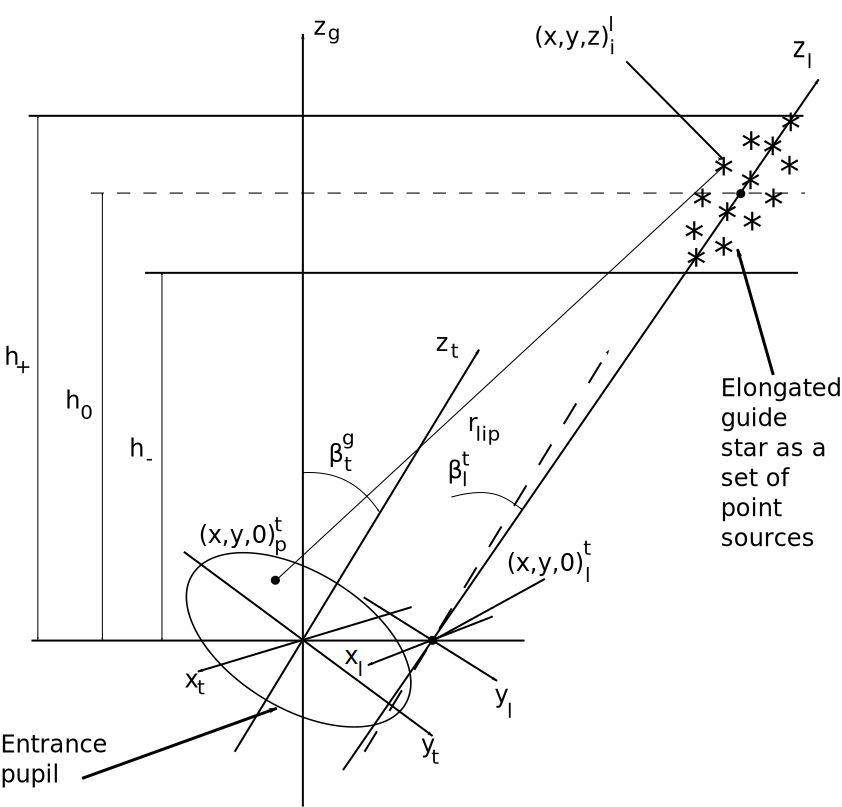
\includegraphics[width = 0.7\textwidth]{LGS.png}
\end{center}
\caption{Geometry of laser guide star propagation to the telescope entrance
pupil.}
\label{fig:lgs-geom}
\end{figure}

Three coordinate systems are involved:
\begin{enumerate}
	\item Global or $g$-system is the Cartesian coordinate system with respect
	to which all other coordinate systems are defined. The orientation pair
	$(\bm{o},\mathcal{R})_{g}^{0}$ for this system is just ($\bm{0},\mathcal{I}$).
	\item Telescope or $t$-system is the local Cartesian coordinate system
	rotating with respect to the $g$-system such that the $t$-system $z$-axis is
	always along the telescope optical axis. The orientation pair
	$(\bm{o},\mathcal{R})_{t}^{g}$ for this system describes the telescope
	pointing. If we assume that at zenith pointing the $t$-system coincides with
	the $g$-system, then \\
	\begin{equation} \label{eq:t-origin}
		\bm{o}^{g}_{t} = \bm{o}^{0}_{g} = \bm{0},
	\end{equation}
	\begin{equation} \label{eq:t-rotation}
		\mathcal{R}^{g}_{t} = \texttt{Eu}(\alpha^{g}_{t},\beta^{g}_{t},0),
	\end{equation}
	where Euler angles $\alpha^{g}_{t},\beta^{g}_{t}$ have meaning of the
	telescope azimuth and zenith angles measured with respect to the g-system
	(note the $g$ superscript). The standard Euler rotation is
	\begin{equation} \label{Euler}
		\texttt{Eu}(\alpha,\beta,\gamma) = \mathcal{A}_{z}(\alpha)
		                                   \mathcal{A}_{y}(\beta)
		                                   \mathcal{A}_{z}(\gamma),
	\end{equation}
	$$ \mathcal{A}_{z}(\alpha) = \left[
     \begin{array}{crc}
	     \cos{\alpha} & -\sin{\alpha} & 0 \\
	     \sin{\alpha} & \cos{\alpha} & 0 \\
	     0 & 0 & 1 \\
		 \end{array} \right],
	$$
	$$ \mathcal{A}_{y}(\beta) = \left[
     \begin{array}{rcc}
	     \cos{\beta} & 0 & \sin{\beta} \\
	     0 & 1 & 0 \\
	     -\sin{\beta} & 0 & \cos{\beta} \\
		 \end{array} \right].
	$$
	Coordinates of point $p$ in the entrance pupil given in $t$-system are
	$[x,y,0]_{p}^{t} = \bm{r}_{p}^{t}$.
	\item Laser launch telescope or $l$-system is a local Cartesian coordinate
	system chosen such that its $z$-axis is always along the optical axis of the
	LLT. This system is naturally defined with respect to the $t$-system because
	the LLT is mounted on the moving main telescope mount:
	\begin{equation} \label{eq:l-system}
		(\bm{o},\mathcal{R})_{l}^{t} = ([x,y,0]_{l}^{t},
                                 \texttt{Eu}(\alpha_{l}^{t},\beta_{l}^{t},0),
	\end{equation}
	where $[x,y,0]_{l}^{t} = \bm{r}_{l}^{t}$ are the $l^{th}$ LLT location in
	$t$-system (pupil
	coordinates), $\alpha_{l}^{t},\beta_{l}^{t}$ are the azimuth and zenith
	angles of the LLT orientation with respect to the main telescope optical
	axis. Note that, for simplicity, we count one LGS per one LLT. In reality
	one LLT of GMT will generate a pair of LGSs. To account for this we simply
	assume that there are two differently oriented virtual LLTs at the location
	of one real LLT.

	The LGS is modeled as a combination of the point sources (PSR) distributed
	within the \texttt{Na} layer. Coordinates
	$\bm{r}_{li}^{l}, \,\, l =
	1,...,\#LLT, \,\, i=1,...,\#PSR$ of the sources are given in the $l$-system.
\end{enumerate}

Given orientation pair $(\bm{o},\mathcal{R})_{b}^{a}$ defining $b$-system
coordinates with respect to $a$-system coordinates, the transformation of
coordinates written in $b$-system into the same coordinates written in
$a$-system is the \emph{direct affine transform}: \index{affine transform}
\begin{equation} \label{eq:direct-affine}
	\bm{r}^{a} = \mathcal{R}_{b}^{a} \bm{r}^{b} + \bm{o}_{b}^{a}.
\end{equation}
Correspondingly, the \emph{inverse affine transform} gives the coordinates
written in $b$-system from the ones written in $a$-system:
\begin{equation} \label{eq:inverse-affine}
	\bm{r}^{b} = (\mathcal{R}_{b}^{a})^{T} (\bm{r}^{a} - \bm{o}_{b}^{a}).
\end{equation}


\subsection{Finding LGS spot elongation and orientation on the detector}
\label{sec:elongation-orientation}

An important geometrical calculation needed for the theoretical evaluation of
the detector noise covariance matrix is to find the parameters of the
elongated LGS image in the detector focal plane.

Let a LGS is produced as a light-emitting column of length $L$ inside the
\texttt{Na} layer. We need to find the length of its image in the
Shack-Hartmann WFS focal plane behind a lenslet with location $\bm{r}^{t}_{l}$
(in the $t$-system)
projected on the telescope entrance pupil and the image orientation with
respect to the detector pixel grid. Let the beginning and end of the LGS light
column have $t$-system coordinates $\bm{r}^{t}_{1}$ and $\bm{r}^{T}_{2}$,
respectively. Consider vectors $\bm{r}^{t}_{1t} =
\bm{r}^{t}_{1}-\bm{r}^{t}_{l}$ and $\bm{r}^{t}_{2t} =
\bm{r}^{t}_{2}-\bm{r}^{t}_{l}$. Then, up to a scaling factor and a possible
mirror flip, the LGS
image on the detector is determined by a $(\varepsilon,\theta)$-pair, where
$\varepsilon$ is the angular size of the LGS column as seen from the lenslet
center $\bm{r}_{l}^{t}$, that is, the angle between vectors $\bm{r}^{t}_{1l}$
and $\bm{r}^{t}_{2l}$, and $\theta$ is the angle
between the $t$-system x-axis and the line of intersection of the $t$-system
xy-plane and the plane made by vectors $\bm{r}^{t}_{1l}$ and $\bm{r}^{t}_{2l}$.
Vectors $\bm{r}_{1,2}$ are most conveniently definable in the $l$-system,
where
\begin{equation} \label{eq:lgs-ends-l}
	\bm{r}^{l}_{1,2} = [0 \, 0 \, z^{l}_{1,2}]^{T}.
\end{equation}
The transformation to $t$-system is
\begin{equation} \label{eq:lgs-ends-t}
	\bm{r}^{t}_{1,2} = \mathcal{R}^{t}_{l} \bm{r}^{l}_{1,2} + \bm{o}^{t}_{l}.
\end{equation}
Using scalar and vector products we get
\begin{eqnarray} \label{eq:epsilon-theta}
	\hat{\bm{r}}^{t}_{1,2} = \frac{\bm{r}^{t}_{1,2}}{|\bm{r}^{t}_{1,2}|}, \\
	\cos \varepsilon = \hat{\bm{r}}^{t}_{1} \cdot \hat{\bm{r}}^{t}_{2}, \\
	\bm{p}^{t}_{12} = \hat{\bm{r}}^{t}_{1} \times \hat{\bm{r}}^{t}_{2}, \\
	\sin \varepsilon = |\bm{p}^{t}_{12}|, \\
	\hat{\bm{p}}^{t}_{12} = \frac{\bm{p}^{t}_{12}}{\sin \varepsilon}, \\
	\hat{\bm{x}}^{t} = [1 \, 0 \, 0]^{T}, \\
	\cos \theta = \hat{\bm{x}}^{t} \cdot \hat{\bm{p}}^{t}_{12}, \\
  \sin \theta = | \hat{\bm{x}}^{t} \times \hat{\bm{p}}^{t}_{12} |.
\end{eqnarray}
Note that, since $\varepsilon$ is very small, in order to preserve accuracy,
all calculations need to be done in double precision.

\subsection{Free-space propagation from LGS to telescope entrance pupil}
\label{sec:free-space-propagation}

The electric field $E$ from the LGS on the telescope entrance pupil is the
superposition of spherical waves emitted from each point source (PS) that
makes the elongated laser guide star spot in the \texttt{Na} layer:
\begin{equation} \label{eq:spherical-superposition}
	E_{lp} = \sum_{i=1}^{\#PSR} w_{li} \frac{\exp(i k r_{lip})}{r_{lip}},
\end{equation}
where $w_{li}$ is the weight describing relative intensity of the $i^{th}$ PS
of the $l^{th}$ LGS, $r_{lip}$ is the distance from the $i^{th}$ PS
of the $l^{th}$ LGS to $p^{th}$ point in the telescope entrance pupil. This
distance is easily found through the affine transform:
\begin{equation} \label{eq:source-to-pupil}
	\bm{r}_{li}^{t} = \mathcal{R}_{l}^{t} \bm{r}_{li}^{l} + \bm{o}_{l}^{t},
\end{equation}
$$ r_{lip} = |\bm{r}_{li}^{t} - \bm{r}_{p}^{t}|. $$

\subsection{Geometrical optics propagation through atmosphere}
\label{sec:geom-propagation}

The turbulent atmosphere on the way between an LGS and a telescope is modeled
as a set of infinitely thin random \emph{phase screens} (PS)
\index{phase screen}. Because of small phase perturbations caused by each
layer and because the typical scale of turbulence is much larger than a
wavelength the geometrical optics model for propagation through the layers is
assumed. The model is based on the following postulates:
\begin{itemize}
	\item The propagation of the electromagnetic waves is treated as propagation
	of \emph{rays} that are normals to the constant phase surfaces of the waves,
	the \emph{wavefronts}. \index{ray} \index{wavefront}
	\item Rays are always straight: the phase screens are weak enough for not
	to change direction of rays, they only add a path difference
	$\delta r_{lip,j}$:
	\begin{equation} \label{eq:path-diff}
		\delta r_{lip,j} = \phi_{lip,j}/k, \,\, j = 1,...,\#PS,
	\end{equation}
	$$ r_{lip}^{turb} = r_{lip}^{free} + \sum_{j=1}^{\#PS} \delta r_{lip,j}. $$
	where $\phi_{lip,j}$ is the phase on the $j^{th}$ turbulent layer
	intersected by a ray emitting from $i^{th}$ point source of $l^{th}$ LGS
	towards $p^{th}$ point in the entrance pupil. So, the electric field
	on the entrance pupil will be
	\begin{equation} \label{eq:spherical-superposition-turb}
		E^{turb}_{lp} =
		\sum_{i=1}^{\#PSR} w_{li}
		\frac{\exp(i k r_{lip}^{turb})}{r_{lip}^{free}}.
	\end{equation}
\end{itemize}

Thus, it is necessary to find the intersection of a ray with a turbulent layer.

\subsubsection{Turbulence layers are perpendicular to the telescope optical
axis.}

Assume that the turbulence layers are chosen such that they are perpendicular
to the telescope optical axis regardless of the pointing.
In this case the turbulence strength depends on the azimuth angle
$\beta_{t}^{g}$, namely,
\begin{equation} \label{eq:turb-vs-beta}
	C_{n}^{2} (\beta_{t}^{g}) = \frac{C_{n}^{2}(0)} {\cos \beta_{t}^{g}}.
\end{equation}

Simple geometrical analysis gives for the
relationship between the pupil and turbulence layer coordinates:
\begin{equation} \label{eq:pupil-to-layer}
  \bm{r}^{t}_{lip,j} =
  \frac{h_{j}}{z^{t}_{li}} \bm{r}_{p}^{t} +
  (1-\frac{h_{j}}{z^{t}_{li}})
  \left[
  \begin{array}{c}
	  x^{t}_{li} \\
	  y^{t}_{li} \\
	  0
	\end{array}
  \right], \,\,
  \bm{r}^{t}_{li} =
  \left[
  \begin{array}{c}
	  x^{t}_{li} \\
	  y^{t}_{li} \\
	  z^{t}_{li}
	\end{array}
  \right],
\end{equation}
where $h_{j}$ is distance between the telescope and $j^{th}$ phase screen
along the telescope optical axis,
$\bm{r}^{t}_{lip,j}$ are xyz-coordinates in $t$-system of an
intersection point on phase screen $j$ for a ray emitting from $i^{th}$ point
source of $l^{th}$ LGS with $t$-coordinates $\bm{r}^{t}_{li}$ and
passing through $p^{th}$ point in telescope entrance pupil with $t$-coordinates
$\bm{r}^{t}_{p}$. For the source at infinity (a natural guide star or a
scientific target) Eq. (\ref{eq:pupil-to-layer}) simplifies to
\begin{equation} \label{eq:pupil-to-layer-inf}
	\bm{r}^{t}_{lip,j} =
	\left[
	\begin{array}{c}
		\cos \alpha^{t}_{li} \\
		\sin \alpha^{t}_{li} \\
		0 \\
	\end{array}
	\right] h_{j} \tan \beta^{t}_{li} + \bm{r}^{t}_{p},
\end{equation}
where $(\alpha,\beta)^{t}_{li}$ are the angular coordinates (first and second
Euler angles) of the light source. Note that in both cases the position of the
ray intersection with a layer can be written as $ (a \bm{r}_{p}^{t} +
\bm{b}^{t}_{li}) $.

\subsubsection{Turbulence layers are parallel to the ground.}

Assume that the layers are parallel to the ground, i.e. perpendicular to the
$g$-system's $z$-axis, and have altitudes $h_{j}, \,\, j = 1,...,\#PS$. In
this case the turbulence $C_{n}^{2}$ profile is not altered with the zenith
angle. Direct ray tracing technique is used to find intersection with a
turbulence layer.

Coordinates of a ray can be described through the parametric equation:
\begin{equation} \label{eq:ray-equation}
	\bm{r}(t) = \bm{i} t + \bm{r}_{0},
\end{equation}
where $\bm{r}_{0}$ is the ray origin (position of the light-emitting source),
$\bm{i}$, $|\bm{i}| = 1$ is the ray
direction vector, $t$ is the ray path length. In the case of propagation path
shown of Fig. \ref{fig:lgs-geom}
$$ \bm{r}^{l}_{0} = \bm{r}^{l}_{li}, $$
where $\bm{r}_{0}$ is given in $l$-system,
$$ \bm{i}^{t} = \frac{\bm{r}^{t}_{p} - \bm{r}^{t}_{li}}
                 {|\bm{r}^{t}_{p} - \bm{r}^{t}_{li}|}, $$
where $\bm{i}$ is given in $t$-system. Since the turbulent layers are most
conveniently defined in the $g$-system, the ray coordinates need to be
transformed into $g$-system:
\begin{equation} \label{eq:ray-transform}
	\bm{r}^{t}_{0} = \mathcal{R}_{l}^{t} \bm{r}^{l}_{0} + \bm{o}_{l}^{t},
\end{equation}
$$ \bm{i}^{t} = \frac{\bm{r}^{t}_{p} - \bm{r}^{t}_{0}}
                 {|\bm{r}^{t}_{p} - \bm{r}^{t}_{0}|}, $$
$$ \bm{r}^{g}_{0} = \mathcal{R}_{t}^{g} \bm{r}^{t}_{0} + \bm{o}_{t}^{g}, $$
$$ \bm{i}^{g} = \mathcal{R}_{t}^{g} \bm{i}^{t}. $$
The coordinates of ray intersection with turbulent layer are found by equating
$z$-coordinate of a ray to the layer altitude:
\begin{equation} \label{eq:layer-intersection}
	t = \frac{h_{j}-r^{g}_{0z}}{i^{g}_{z}},
\end{equation}
$$ \bm{r}^{g}_{lip,j} = \bm{i}^{g} t + \bm{r}_{0}^{g}, $$
where $x$- and $y$-coordinates of the $\bm{r}^{g}_{lip,j}$-vector are used to
find the phase $\phi^{turb}(\bm{r}^{g}_{lip,j}) = k \delta r^{turb}_{lip,j}
(\bm{r}^{g}_{lip,j})$ on the phase
screen corresponding to the ray intersection and substitute it to Eq.
(\ref{eq:spherical-superposition-turb}).


\subsection{Point source distribution in the LGS}
\label{sec:point-distribution}
TBC

The positions $\bm{r}^{l}_{li}$ and weights $w_{li}$ of point sources making
each LGS are found from superposition of the intensity distribution of the laser
radiation forward-propagated through atmosphere to the \texttt{Na} layer and
the vertical distribution of the \texttt{Na} density. A possible operation
flow for defining the LGS distribution is the following:
\begin{enumerate}
	\item Define a 3D mesh covering a part of the \texttt{Na} layer penetrated
	by the laser radiation. Each cell of this mesh is an elementary volume for
	which amount of laser flux is assigned.
	\item Center of each 3D mesh cell is the candidate location of the LGS point
	source. If flux through the cell exceeds a threshold, a point source is
	assigned for this cell.
	\item For each mesh cell for which a point source is assigned multiply the
	cell flux by \texttt{Na} density at the cell center taken from the
	\texttt{Na} vertical profile. Find relative distribution of the return flux,
	which is the source weights $\{ w_{li} \}_{i=1}^{\#PSR}$:
	\begin{equation} \label{eq:source-weights}
		w_{li} = \frac{ \Phi_{li} C^{\texttt{Na}}_{li} }
		               { \sum_{i=1}^{\#PSR} \Phi_{li} C^{\texttt{Na}}_{li} },
		           \,\, i = 1, ... , \#PSR
	\end{equation}
	where $\{ \Phi_{li} \}_{i=1}^{\#PSR}$ are the cell fluxes,
	$\{ C^{\texttt{Na}}_{li} \}_{i=1}^{\#PSR}$ are the \texttt{Na} abundances at
	the cell locations.
\end{enumerate}

\subsection{Return flux in the entrance pupil}
\label{sec:return-flux}

The photon flux returning from each LGS point source is considered uniformly
distributed over the spherical surface of the wavefront. Since the solid angle
$\Omega$ at which the telescope is seen from the source is typically very
small, the variation of $r^{free}_{lip}$ in the denominator of Eq.
(\ref{eq:spherical-superposition-turb}) over the pupil can be neglected. Thus,
the fraction of energy emitting from a point source that passes through the
telescope entrance pupil is
\begin{equation} \label{eq:energy-fraction}
	\frac{\Omega}{4 \pi} = \frac{1}{4 \pi}
	\frac{ A_{p} }
	     { |\bm{r}^{t}_{li}|^{2} \cos^{2} \beta^{t}_{li} },
\end{equation}
where $A_{p}$ is the pupil area, $|\bm{r}^{t}_{li}|$ is the distance from
pupil center to the point source, $\beta^{t}_{li}$ is the angle between the
telescope optical axis and the direction to the point source as seen from the
pupil center,
\begin{equation} \label{eq:angle-to-source}
	\cos \beta^{t}_{li} = \left( \frac{\bm{r}^{t}_{li}}
	                                  {|\bm{r}^{t}_{li}|} \right)_{z}.
\end{equation}
The photon flux into the entrance pupil from a point source is
\begin{equation} \label{eq:return-flux}
	\Phi_{li} = \tau T_{AOS} \frac{T_{ATM}}{\cos{\beta^{g}_{li}}}
	            s^{\texttt{Na}} C^{\texttt{Na}}
	            P_{l} w_{li}
	            \frac{\Omega}{4 \pi}, \,\, [\texttt{photons}],
\end{equation}
where \\
\begin{tabular}{lcll}
	&&& \\
  Exposure time & : & $\tau$ & = 2 ms, \\
  Atmosphere transmittance & : & $T_{ATM}$ & = 0.89, \\
  AO system transmittance & : & $T_{AOS}$ & = 0.448, \\
  Sodium coupling efficiency & : & $s^{\texttt{Na}}$ &
  = 130 (photons m$^{2}$ )/(s W atom), \\
  Sodium abundance & : & $C^{\texttt{Na}}$ & = $2.1\times10^{13}$ atoms/m$^2$,\\
	Laser power per LGS & : & $P_{l}$ & = 20 W, \\
	&&& \\
\end{tabular} \\
$\beta^{g}_{li}$ is the angle between zenith direction and the point source
direction as viewed from the entrance pupil center.

The fluxes from all point sources are later summed on the detector.
% To be compiled with pdf LaTeX
% This file is to be included into master file via \input command
% Note that there is no \begin{document} \end{document} brackets!

\newpage
\section{Shack-Hartmann Wavefront sensor modeling}
\label{sec:sh-wfs}

\mbox{}

\subsection{Nomenclature}

\mbox{}

$\bm{s} = (s_{x},s_{y})$ - vector of xy-slope measurements read from one
Shack-Hartmann sensor subaperture, [m or pixels].
\\

$I(x,y)$ - intensity distribution in the detector focal plane, [].
\\

$\langle \bm{s} \bm{s}^{T} \rangle - \langle \bm{s} \rangle
\langle \bm{s} \rangle^{T}$ - covariance matrix of the xy-slope measurements,
[m$^{2}$ or pixel$^{2}$].
\\

$A$ - area of subaperture, [m$^{2}$].
\\

$p$ - detector pixel size, [m].
\\

$n_{ph}$ - number of photons passed through a subaperture, [].
\\

$\sigma_{e}$ - readout noise, [electrons/pixel].
\\

$f_{L}$ - lenslet focal distance, [m]
\\

$\Gamma_{L}$ - angular magnification in the detector exit pupil, [].
\\

$\varepsilon_{Na}$ - angular fwhm size of \texttt{Na} LGS projected to sky as
seen from a subaperture, [rad].
\\

$\varepsilon_{0}$ - angular fwhm size of a point source projected to sky as
seen from a subaperture, [rad].
\\

$\theta_{e}$ - orientation angle of the elongated spot on the detector, [rad].

\subsection{Sensor geometry}
\label{subsec:sh-wfs-geometry}

TBD

\subsection{Propagation from exit pupil to detector}
\label{subsec:sh-wfs-propagation}

\mbox{}

The sampling of the pupil is derived from the sampling in the WFS detector
focal plane.
If $n_d$ is the number of samples across each spot on the detector and the
fwhm of the
diffraction limited spot is sampled with $k$ pixels, then the pupil sampling is
$2Nn_d/k=Nn$, where $N$ is number of subapertures across the pupil diameter,
$n$ is number of pixels across a subaperture diameter.
It is required that either $k$ or $1/k$ is an integer and that $k\leq 2$.
It is worth nothing that a field stop the size of a subaperture
field--of--view is assumed.
The pixel scale  and the field--of--view are given by $\lambda/dk$ and
$n_d\lambda/dk$, respectively, with $\lambda$ the wavefront sensing
wavelength and $d$ the lenslet pitch.

The Shack--Hartmann wavefront sensor (SH--WFS) model
\begin{enumerate}
\item the telescope pupil $\Pi$ is cut in $N\times N$ square pieces of
$n\times n$ pixels corresponding to the $N\times N$ lenslet array, for the
lenslet $(k,l)$ this is $$a_{kl} =
\Pi[kn,\dots,(k+1)n-1][ln,\dots,l(n+1)-1]\quad k,l=0,\dots,N-1,$$
\item each square array is multiplied by a complex phase ramp to keep the
spot at the center of the array in the free aberration case,
$$a_{kl}^\prime(i,j) = a_{kl}(i,j)\exp(\iota \pi (i+j)(n-1)/n^\prime)\quad
i,j=0,\dots,n-1$$ with $n^\prime=2n$ if $n$ is even or  $n^\prime=2n+1$ if $n$
 is odd and $\iota=\sqrt{-1}$,
\item each square array is padded with zeros in both directions up to
$n^\prime$,$$a_{kl}^\prime[n,\dots,n^\prime-1][n,\dots,n^\prime-1]=0,$$
\item a discrete Fourier transform is performed on each zero--padded array,
$$\tilde a_{kl}^\prime = DFT\left\{a_{kl}^\prime\right\},$$
\item each resulting array is reduced to half its size, $$\tilde a_{kl} =
\tilde a_{kl}^\prime[0,\dots,n-1][0,\dots,n-1],$$
\item the spot intensities are computed from the squared modulus of the
reduced arrays, $$b_{kl} = \left| \tilde a_{kl} \right|^2,$$
\item if needed i.e. $k<2$, the intensity map are binned to the detector
array size, $$b_{kl}^\prime(k,l) =
\sum_{i=kn_d}^{(k+1)n_d-1}\sum_{j=ln_d}^{(l+1)n_d-1} b_{kl}(i,j)\quad
k,l=0,\dots,n_d-1 $$
\end{enumerate}

\subsection{Centroiding methods}
\label{subsec:sh-wfs-centroid}

The four spot centroiding methods are considered for the GMT LTAO Shack-Hartmann
sensors:
\begin{enumerate}
	\item \emph{Center of Gravity}: \index{Center of Gravity centroid}
	\begin{equation} \label{eq:CoG}
	\left[ \begin{array}{c} s_{x} \\ s_{y} \end{array} \right] =
	\frac{1}{\sum_{xy} I(x,y)}
	\sum_{xy} \left[ \begin{array}{c} x \\ y \end{array} \right] I(x,y),
	\end{equation}
	where $\bm{s} = (s_{x},s_{y})$ is the slope readout from the spot,
	$I(x,y)$ is the intensity distribution read out from detector pixels,
	summation is done over the pixels in the area occupied by a single spot.
	\item \emph{Weighted Center of Gravity} \index{Weighted Center of Gravity
	centroid} is the Center of Gravity algorithm
	applied to image $I(x,y) I_{0}(x,y)$, where $I_{0}(x,y)$ is a
	\emph{reference image}. \index{reference image}
	\item \emph{Correlation} \index{Correlation centroid} algorithm finds spot
	position as that of maximum of the correlation function
	\begin{equation} \label{eq:corr}
		C(\bm{s}) = \sum_{xy} I(x,y) I_{0}(x-s_{x},y-s_{y}),
	\end{equation}
	where $I_{0}(x,y)$ is a reference image.
	\item \emph{Quad cell} \index{quad cell} centroiding algorithm is used in
	the tip/tilt WFS, which has 4 pixels per spot. The quad cell readout is
	\begin{equation} \label{eq:quad-cell}
		s_{x} = \frac{1}{\sum_{i=1}^{4} I_{i}} (I_{1} + I_{2} - I_{3} - I_{4}),
	\end{equation}
	$$
		s_{y} = \frac{1}{\sum_{i=1}^{4} I_{i}} (I_{1} + I_{3} - I_{2} - I_{4}),
	$$
	where $\{ I_{i} \}_{i=1}^{4}$ are the four intensity reads from the quad
	cell pixels.
\end{enumerate}
Discussion of these centroiding approaches is given in Ref.
\cite{ConanCentroid}.

\subsection{Sensor noise covariance matrix}
\label{subsec:sh-wfs-noise-covariance}

\mbox{}

This section describes the derivation of the noise covariance matrix for a
SH--WFS with a $N_L\times N_L$ lenslet array paving a telescope pupil of
diameter $D$.
The spots of the SH--WFS are assumed to be seeing
limited i.e. $r_0<D/N_L$, $r_0$ is the Fried parameter. Thus, the projected to
sky angular size of the spot formed by a lenslet is
$\varepsilon_0=\lambda/r_0$, $\lambda$ is the WFS operational wavelength.
The spot elongation due to elongated LGS is characterized by the
$(\varepsilon_{Na},\theta_{e})$-pair of the fwhm angular size
along the \texttt{Na} LGS elongation direction and the elongation
orientation angle. Both these parameters depend on the mutual orientation
lenslet and the LLT, altitude and thickness of the \texttt{Na} layer, and the
LLT pointing. The calculation of the $(\varepsilon_{Na},\theta_{e})$-pair is
described in Section \ref{sec:elongation-orientation}.

The spot intensity profile due to the LGS is
assumed to be Gaussian with elliptical cross section and the long ellipse axis
is rotated by angle $\theta_{e}$ with respect to the camera focal plane
xy-coordinates:
\def\nph{n_{ph}}
\begin{equation}
  \label{eq:2}
  I_{S}(x,y) = { \nph \over 2\pi \sigma_x\sigma_y }
  \exp\left( - { x^{\prime 2} + y^{\prime 2} \over 2\sigma_x\sigma_y}\right),
\end{equation}
where subscript $S$ stands for the star image distribution,
$\nph$ is the photon flux through the subaperture,
\def\vr{\bm{r}}
\def\vre{\bm{r_e}}
\begin{eqnarray}
  \label{eq:3}
  x^{\prime} &=& x\cos(\theta_e) - y\sin(\theta_e), \\
  y^{\prime} &=& x\sin(\theta_e) + y\cos(\theta_e),
\end{eqnarray}
$\sigma_x$ and $\sigma_y$ are related to the fwhm of the non-elongated and
elongated spot, respectively, as
\begin{eqnarray}
  \label{eq:6}
  \varepsilon_{x,y} &=& 2\sqrt{2\ln(2)}\sigma_{x,y}, \\
  \varepsilon_{x,y} &=& f_{L} \Gamma_{L} \varepsilon_{0,Na},
\end{eqnarray}
where $f_{L}$ is the lenslet focal distance, $\Gamma_{L}$ is the angular
magnification in the exit pupil where the lenslet array is located.

The spot centroid xy-readout in the lenslet focal plane in case of the
\emph{Center of Gravity} centroiding algorithm \index{Center of Gravity
centroid} is given by
\begin{equation}
  \label{eq:10}
  \bm{s} = \left[ \begin{array}{c} s_{x} \\ s_{y} \end{array} \right] =
  \frac{1} {\iint_A I(x,y) {\rm d}x{\rm d}y}
  \iint_A
  \left[ \begin{array}{c} x \\ y \end{array} \right]
  I(x,y) {\rm d}x{\rm d}y,
\end{equation}
where $I(x,y)$ is the complete intensity distribution in the spot that
includes the star intensity disribution and some other additions,
$A=(D/N_L)^2$ is the lenslet area.

\subsection{Spot intensity distribution}
\label{sec:spot-intensity}

To proceed with computation of the spot
readout covariance assumptions about the spot intensity distribution need to
be made:
\begin{enumerate}
	\item The whole intensity distribution is
	\begin{equation} \label{eq:whole-intensity}
		I(x,y) = I_{S}(x,y) + I_{B}(x,y),
	\end{equation}
	where $I_{S}(x,y)$ is given in Eq. (\ref{eq:2}), $I_{e}(x,y)$ is the
	background image due to sensor readout noise.
	\item $I_{S}(x,y)$ and $I_{B}(x,y)$ are statistically independent, i.e.
	$\langle I_{S}(x,y)I_{B}(x,y) \rangle = 0$.
	\item $\langle I_{B}(x,y) \rangle$ = 0.
	\item All the $I_{S}(x,y)$ distribution energy is concentrated inside region
	$A$, so \\ $ \iint_A I_{S}(x,y) {\rm d}x{\rm d}y \approx \nph = const$.
	\item The random process $I_{B}(x,y)$ is ergodic, so
	$0 = \langle I_{B}(x,y)
	\rangle \approx \iint_{A} I_{B}(x,y) {\rm d}x {\rm d}y$, which, together
	with the previous assumption gives
	$ \iint_A I(x,y) {\rm d}x{\rm d}y \approx \nph $.
	\item Spot cross-talk is negligible, so
  spots from different lenslets are statistically independent. Therefore, the
  full WFS readout covariance matrix is block diagonal with 2x2 blocks
  corresponding to each spot xy-slope covariance.
  \item Pixel intensities are statistically independent, i.e.
  $\langle I(x,y)I(x^{\prime},y^{\prime}) \rangle = 0$.
\end{enumerate}
Eq. (\ref{eq:10}) due to assumptions 5, 6 simplifies to
\begin{eqnarray}
  \label{eq:11}
  \bm{s} =
  \frac{1} {\nph}
  \iint_A
  \left[ \begin{array}{c} x \\ y \end{array} \right]
  I(x,y) {\rm d}x{\rm d}y.
\end{eqnarray}
The covariance of the spot centroid readouts is given by
\begin{equation}
  \label{eq:12}
  \langle \bm{s} \bm{s}^{T} \rangle -
  \langle \bm{s} \rangle \langle \bm{s}^{T} \rangle
\end{equation}
$$
  = {1 \over \nph^2} \iint_A \iint_A
  \left[
  \begin{array}{cc} x_{1} x_{2} & x_{1} y_{2} \\
                    y_{1} x_{2} & y_{1} y_{2} \end{array}
  \right]
  ( \langle I(x_{1},y_{1}) I(x_{2},y_{2}) \rangle
  - \langle I(x_{1},y_{1}) \rangle
    \langle I(x_{2},y_{2}) \rangle )
    {\rm d}x_{1}{\rm d}y_{1} {\rm d}x_{2}{\rm d}y_{2}.
$$
Substututing Eq. (\ref{eq:whole-intensity}) and using assumptions 2, 3, and 7
we simplify this equation to
\begin{equation}
  \label{eq:13}
  \langle \bm{s} \bm{s}^{T} \rangle -
  \langle \bm{s} \rangle \langle \bm{s}^{T} \rangle
\end{equation}
$$
 = {1 \over \nph^2} \iint_A{}
   \left[
   \begin{array}{cc}
	   x^{2} & xy    \\
	   xy    & y^{2}
	 \end{array}
   \right]
   (\sigma_{I}^{2}(x,y)+\sigma_{B}^{2})
   {\rm d}x{\rm d}y,
$$
where
$$
  \sigma_{S}^{2}(x,y) =
  \langle I_{S}^{2}(x,y) \rangle - \langle I_{S}(x,y) \rangle^{2},
$$
is the variance distribution in the star intensity distribution,
$$
  \sigma_{B}^{2} = \langle I^{2}_{B}(x,y) \rangle = const.
$$
is the readout noise variance. Thus the sensor readout covariance has two
terms that can be treated independently.

\subsection{Photon noise}
\label{sec:photon-noise}

The photon noise follows a Poisson statistics distribution with variance
$\sigma_{S}^{2}(x,y) = I_{S}(x,y)$.
Thus the spot centroid readouts covariance in the case of
the photon noise is given by
\begin{equation}
  \label{eq:1}
  \langle \bm{s} \bm{s}^{T} \rangle_{S} -
  \langle \bm{s} \rangle_{S} \langle \bm{s}^{T} \rangle_{S}
\end{equation}
$$ = {1 \over \nph^2} \iint_{A}
   \left[
   \begin{array}{cc}
	   x^{2} & xy \\
	   xy    & y^{2}
	 \end{array}
   \right]
   I_{S}(x,y) \;{\rm d}x {\rm d}y,
$$
where $\nph$ is the number of photons per subaperture, $x$ and $y$ are the
coordinates in the focal plane,
the intensity $I_{S}(x,y)$ in the focal plane given by Eq. (\ref{eq:2}).

Substututing Eq.(\ref{eq:2}) into Eq.~(\ref{eq:1}) and performing the
integration leads to
\begin{equation}
  \label{eq:4}
  \langle \bm{s} \bm{s}^{T} \rangle_{S} -
  \langle \bm{s} \rangle_{S} \langle \bm{s}^{T} \rangle_{S}
\end{equation}
$$
  = {1 \over \nph}
  \left[
  \begin{array}{cc}
	  \sigma_{x}^{2} \cos^{2} \theta_{e} + \sigma_{y}^{2} \sin^{2} \theta_{e} &
	  (\sigma_{x}^{2}-\sigma_{y}^{2}) \cos \theta_{e} \sin \theta_{e} \\
	  (\sigma_{x}^{2}-\sigma_{y}^{2}) \cos \theta_{e} \sin \theta_{e} &
	  \sigma_{x}^{2} \sin^{2} \theta_{e} + \sigma_{y}^{2} \cos^{2} \theta_{e}
	\end{array}
  \right]
$$
$$
  =
  \left[
  \begin{array}{cc}
	  \sigma^{2}_{xx} & \sigma^{2}_{xy} \\
	  \sigma^{2}_{xy} & \sigma^{2}_{yy}
	\end{array}
  \right].
$$

From Eq.(\ref{eq:4}), it is obvious that covariance is null when the
spots are oriented either along the x or y axis or if the fwhms of both x and
y axis are the same.

\subsection{Read-out noise}
\label{sec:read-out-noise}

The read-out noise follows a zero-mean
Gaussian distribution of variance $\sigma^{2}_{B} = \sigma^2_e / p^{2}$,
where $\sigma^{2}_{e}$ is the number of read noise electrons squared per
pixel area $p^2$. Since $\sigma^{2}_{B} = const.$ and, with assumption that $A$
is a square lenslet, we have
$$
  \sigma^{2}_{B} \iint_{A} xy {\rm d}x{\rm d}y = 0,
$$
$$
  \iint_{A} x^{2} {\rm d}x{\rm d}y =
  \iint_{A} y^{2} {\rm d}x{\rm d}y.
$$
Thus the readout noise covariance matrix is diagonal:
\begin{equation} \label{eq:14}
	\langle \bm{s} \bm{s}^{T} \rangle_{B} =
	\left[{}
	\begin{array}{cc}
		\sigma^{2}_{ron} & 0 \\
		0 & \sigma^{2}_{ron} \\
	\end{array}
	\right].
\end{equation}
For a square lenslet of size $d=D/N_L$ we get
\begin{equation} \label{eq:15}
     \sigma_{ron}^2 = \left(\sigma_e \over p \nph \right)^2
     \int_{-d/2}^{d/2} \int_{-d/2}^{d/2} x^2 {\rm d}x{\rm d}y \\
                   = {1\over 12}\left(d^2\sigma_e \over p \nph \right)^2 =
                   {N_d^2\over 12}\left(D\sigma_e \over N_L \nph \right)^2,
\end{equation}
$N_d$ is the total number of pixels used for computing the centroids.

Finally, the sensor readout
noise covariance matrix for one lenslet is a sum of covariance matrices for
photon and readout noises:
\begin{equation}
  \label{eq:16}
  \langle \bm{s} \bm{s}^{T} \rangle_{S+B} -
  \langle \bm{s} \rangle_{S+B} \langle \bm{s}^{T} \rangle_{S+B} =
  \left[
    \begin{array}{cc}
      \sigma^2_{xx} + \sigma_{ron}^2 & \sigma_{xy} \\
      \sigma_{xy} & \sigma^2_{yy} + \sigma_{ron}^2
    \end{array}
  \right].
\end{equation}
For the whole lenslet array, the noise covariance matrix is a block diagonal
with these matrices on the diagonal.
% To be compiled with pdf LaTeX
% This file is to be included into master file via \input command
% Note that there is no \begin{document} \end{document} brackets!

\newpage
\section{Deformable mirror modeling}
\label{sec:dm}


\subsection{Nomenclature}

TBD

\subsection{Deformable mirror geometry}
\label{subsec:dm-geometry}

TBD

\subsection{Linear model}
\label{subsec:dm-linear-model}


\subsection{Influence functions}
\label{subsec:dm-influence}

TBD

\subsection{Fitting error}
\label{subsec:dm-fitting-error}

TBD

\subsection{Internal dynamics}
\label{subsec:dm-dynamics}

TBD
% To be compiled with pdf LaTeX
% This file is to be included into master file via \input command
% Note that there is no \begin{document} \end{document} brackets!

\newpage
\section{Control}
\label{sec:control}

%\subsection{Nomenclature}

%\mbox{}

%$\bm{s}$ - vector of wavefront sensor measurements concatenated both for x- and
%y-slopes and from different sensors, [pixels or radians of slope].
%\\

%$\phi(\bm{x})$ - continuous wavefront phase distribution in exit pupil, [rad].
%\\

%$\{ \phi(\bm{x})_{i} \}_{i=1}^{\infty}$ - set of basis functions for the exit
%pupil phase expansion, [rad].
%\\

%$\bm{x}_{Sc}$ - vector of discretized phase values in the telescope exit pupil
%for the light coming from a science object, [rad].
%\\

%$\hat{\bm{x}}_{0}$ - estimate of vector of discretized phase values in the
%telescope exit pupil
%for the light coming from a science object, [rad].
%\\

%$\bm{x}$ - vector of discretized phase values in the telescope exit pupil for
%the light from a guide star to wavefront sensor, concatenated for all sensors,
%[rad].
%\\

%$\bm{n}_{s}$ - vector of sensor readout noise concatenated from all sensors,
%[pixels or radians of slope].
%\\

%$\{ f(\bm{x})_{i} \}_{i=1}^{\#actuators}$ - set of continuous phase influence
%functions of a deformable mirror, [rad].

%$\bm{c}$ - vector of control commands concatenated from all correctors (DMs,
%tip-tilt mirrors, moving stages), [control units, e.g. V].
%\\

%$\hat{\bm{c}}$ - vector of control commands estimated from a control algorithm.
%\\

%$\bm{n}_{a}$ - vector of actuator noise concatenated from all correctors,
%[control units].
%\\

%$\mathcal{E}$ - estimation (control) matrix.
%\\

%$\mathcal{G}$ - wavefront-to-WFS interaction matrix, [rad/slope].
%\\

%$\delta \mathcal{G}$ - error in the wavefront-to-WFS interaction matrix,
%[rad/slope].
%\\

%$\mathcal{D}$ - command-to-WFS interaction (``poke'') matrix, [control
%units/slope].
%\\

%$\delta \mathcal{D}$ - error in the command-to-WFS interaction matrix,
%[rad/slope].
%\\

%$\mathcal{F}$ - command-to-phase interaction (``influence function'') matrix,
%[control units/rad].
%\\

%$\delta \mathcal{F}$ - error in command-to-phase interaction (``influence
%function'') matrix, [control units/rad].
%\\

%$\langle \bm{x} \bm{x}^{T} \rangle$ - auto-covariance matrix of the guide star
%phase in exit pupil, [rad$^{2}$].
%\\

%$\langle \bm{x}_{Sc} \bm{x}^{T} \rangle$ - cross-covariance matrix of the
%science object and guide star phase in exit pupil, [rad$^{2}$].
%\\

%$\langle \bm{n}_{s} \bm{n}_{s}^{T} \rangle$ - auto-covariance matrix of the
%sensor readout noise, [slope$^{2}$].
%\\

%$\langle \bm{n}_{a} \bm{n}_{a}^{T} \rangle$ - auto-covariance matrix of the
%actuator noise, [control units$^{2}$].
%\\

\subsection{Linear system model and discretization}
\label{subsec:system-models}

In our treatment of an AO system modeling we follow closely the ``natural
modeling'' approach described in Refs.
\cite{WibergMaxGavel1,WibergMaxGavel2}. To begin with, we consider the simplest
case of a single-conjugate AO system, which is modeled through the following
fundamental inputs.
\begin{enumerate}
	\item A light source to be imaged with an AO system (the \emph{target})
	creates a continuous phase distribution $\phi_{0}(\bm{x})$ in the
  telescope entrance pupil,
	which is the accumulated phase distortion along the
  path from a light source to the telescope that includes atmospheric
  turbulence distortion. It is supposed that the
  autocorrelation function $\langle \phi_{0}(\bm{x}_{1}) \phi_{0}(\bm{x}_{2})
  \rangle_{\phi}$ is known.
  \item A set $\{ f_{i}(\bm{x}) \}_{i=1}^{\#ACT}$ ($\#ACT$ is the number of DM
  actuators) of the DM actuator influence
  functions projected as phase correction in the telescope entrance pupil. We
  will write these functions in vectorial form $\bm{f}(\bm{x})$. Note that, same
  as $\phi(\bm{x})$, these functions depend on the light source. The DM
  correction is assumed to be a linear combination of the influence functions:
  \begin{equation} \label{eq:dm-phase-correction}
		\phi_{DM}(\bm{x}) = \sum_{i=1}^{\#ACT} c_{i} f_{i}(\bm{x})
	\end{equation}
	or
	$$
	  \phi_{DM}(\bm{x}) = \bm{f}^{T}(\bm{x}) \bm{c},
	$$
	where $\bm{c}$ is the vector of DM correction commands.
  \item A wavefront sensor (WFS) accepts light from a \emph{reference} source
  not in general coinciding with the target. WFS is modeled as a linear
  mapping of the reference wavefront $\phi{x,y}$ in the entrance pupil to a
  set of sensor measurements:
  \begin{equation} \label{eq:wfs-measurement-operator}
    \bm{s} = \mathcal{M} [ \phi(\bm{x}) ],
  \end{equation}
  where $\mathcal{M}$ is a linear \emph{measurement operator}.
  \index{measurement operator} The \emph{measurement equation}
  \index{measurement equation} describing the full linear sensor model is
  \begin{equation} \label{eq:measurement-equation}
	  \bm{s} = \mathcal{M} [ \phi(\bm{x}) + \delta \phi(\bm{x}) ] + \bm{n},
  \end{equation}
  where $\bm{n}$ is random sensor readout noise with known autocorrelation
  matrix $\langle \bm{n} \bm{n}^{T} \rangle_{n}$,
  $\delta \phi(\bm{x})$ is an additive aberration due to propagation from
  telescope entrance pupil to the exit pupil conjugate to the WFS location. We
  will assume for the moment that this aberration can be perfectly calibrated
  out, so $\delta \phi (\bm{x}) = 0$.
\end{enumerate}
This small set of parameters are enough to fully describe a linear model of an
AO system.

\subsection{Minimum Mean Square Error AO control}
\label{subsec:MMSE-control}

The goal of the \emph{Minimum Mean Square Error} (MMSE) \index{Minimum Mean
Square Error} AO control is to find a command vector $\hat{\bm{c}}$ such that
the DM correction minimizes the target wavefront mean square phase error
(\emph{quadratic cost}) \index{quadratic cost} in the
telescope entrance pupil
\begin{equation} \label{eq:mmse-cost}
	\langle J \rangle_{\phi,n} =
	\langle ||\phi_{0}-\phi_{DM}||^{2} \rangle_{\phi,n},
\end{equation}
where Hilbert space norm
\begin{equation} \label{eq:Hilbert-norm}
	|| a(\bm{x}) ||^{2} = [a(\bm{x}),a(\bm{x})] =
	\frac{1}{|A|} \int_{A} ds \, a^{2}(\bm{x}),
\end{equation}
is derived from the Hilbert space metric
\begin{equation} \label{eq:Hilbert-metric}
	[a(\bm{x}),b(\bm{x})] = \frac{1}{|A|} \int_{A} ds \, a(\bm{x}) b(\bm{x}),
\end{equation}
$A$ is the telescope entrance pupil domain (the \emph{aperture}),
\index{aperture} $|A|$ is the aperture area, and $\langle \rangle_{\phi}$
denotes averaging over joint statistics of the input turbulent wavefront and
the sensor noise. We can consider two cases of the quadratic cost
minimization: 1) \emph{DM fitting} \index{DM fitting} and 2) \emph{phase
estimation}. \index{phase estimation}

\subsubsection{DM fitting}

The DM fitting problem statement is:
given target wavefront phase $\phi_{0}(\bm{x})$ at the entrance pupil find the
DM command vector $\hat{\bm{c}}$ such that the deterministic wavefront error
is minimized:
\begin{equation} \label{eq:DM-fit-minimization}
	\hat{\bm{c}} = \arg \min_{\forall \bm{c}}
	||\phi_{0} - \bm{f}^{T} \bm{c}||^{2}.
\end{equation}
It is known from the theory of Hilbert spaces that the above equation is
equivalent to
\begin{equation} \label{eq:deterministic-orthogonality-principle}
	[\phi_{0} - \bm{f}^{T} \hat{\bm{c}}, \bm{f}] = 0,
\end{equation}
which is a form of the \emph{orthogonality principle} stating that
\begin{flushleft}
	\texttt{the optimal fitting error is orthogonal to the subspace spanned by
	the influence functions.}
\end{flushleft}
Solving Eq. (\ref{eq:DM-fit-minimization}) or the equivalent Eq.
(\ref{eq:deterministic-orthogonality-principle}) yields for the optimal
control command
\begin{equation} \label{eq:fitting-commands}
	\hat{\bm{c}} = [\bm{f},\bm{f}^{T}]^{\dagger} [\bm{f},\phi_{0}],
\end{equation}
where $[\bm{f},\bm{f}^{T}]$ is called \emph{Gramm matrix} of the function set
$\bm{f}(\bm{x})$, $^{\dagger}$ stands for pseudo inverse. The Gramm matrix is
square and is invertible in case the influence functions $\bm{f} (\bm{x})$ are
linearly independent. Since linear independence is not guaranteed for the real
DM influence functions, the filtered pseudo-inverse is used. Note that in case
of pseudo-inverse the orthogonality principle does not hold exactly. This,
however, is easily fixed if we redefine the influence functions as, e.g., a
subset of orthogonal singular modes of the Gramm matrix with sufficiently large
singular values.

The optimal \emph{fitting error} is \index{fitting error}
\begin{equation} \label{eq:fitting-error}
	J_{c} = [\phi_{0} - \bm{f}^{T} \hat{\bm{c}},\phi_{0} -
	         \bm{f}^{T} \hat{\bm{c}}]
\end{equation}
$$
  = [\phi_{0} - \bm{f}^{T} \hat{\bm{c}},\phi_{0}]
$$
$$
  = [\phi_{0},\phi_{0}] -
    [\bm{f}^{T},\phi_{0}] [\bm{f},\bm{f}^{T}]^{\dagger} [\bm{f},\phi_{0}],
$$
where we used Eqs. (\ref{eq:deterministic-orthogonality-principle}) and
(\ref{eq:fitting-commands}). The orthogonality principle states that the phase
can be presented as a sum of two mutually orthogonal \emph{controllable}
$\hat{\phi}_{0}$ and
\emph{uncontrollable} $\check{\phi}_{0}$ parts \index{controllable part}
\index{uncontrollable part}
\begin{equation} \label{eq:controllable-uncontrollable}
	\phi (\bm{x}) = \hat{\phi}_{0} (\bm{x}) + \check{\phi}_{0} (\bm{x}),
\end{equation}
where
\begin{equation} \label{eq:controllable-projection}
	\hat{\phi}_{0} = \bm{f}^{T} [\bm{f},\bm{f}^{T}]^{\dagger} [\bm{f},\phi_{0}] =
	\mathcal{F} \phi_{0},
\end{equation}
\begin{equation} \label{eq:uncontrollable-projection}
	\check{\phi}_{0} = \phi_{0} - \mathcal{F} (\phi_{0}) =
	(\mathcal{I - F})\phi_{0}
\end{equation}
and $\mathcal{F},\mathcal{I - F}$ are orthogonal projection operators on,
respectively, \emph{controllable} and \emph{uncontrollable subspaces} of the
influence function set $\bm{f}$. \index{controllable subspace}
\index{uncontrollable subspace} Note that the dimension of the controllable
subspace is finite, so either $\hat{\bm{c}}$ or $\bm{\phi}_{0} =
[\bm{f},\phi_{0}]$
are the natural discrete representations for the controllable part of the
wavefront phase, the only part of interest in the AO control.

\subsubsection{Phase estimation}

The phase estimation problem statement is: given sensor measurements $\bm{s}$
find an estimate $\tilde{\phi}_{0}(\bm{x})$ of the target source phase in the
entrance pupil such
that the mean square error is minimized over the measurement statistics, in
our case, the joint turbulence and sensor noise statistics:
\begin{equation} \label{eq:estimation-minimization}
	\tilde{\phi}_{0} =
	\arg \min_{\forall \mathcal{E}}
	\langle
	||\phi_{0} - \mathcal{E} \bm{s}||^{2}
	\rangle_{\phi,n},
\end{equation}
where $\mathcal{E}$ is the linear estimator operator.
Analogously to the deterministic orthogonality principle the \emph{orthogonality
principle of statistical estimation} \index{orthogonality principle} states that
\begin{flushleft}
	\texttt{optimal estimator error is statistically orthogonal to the
	measurements,}
\end{flushleft}
i.e., for our case
\begin{equation} \label{eq:statistical-orthogonality-principle}
	\langle ( \mathcal{E}\bm{s} - \phi_{0} ) \bm{s}^{T} \rangle_{\phi,n} = 0.
\end{equation}
Solving Eq. (\ref{eq:estimation-minimization}) or its equivalent
(\ref{eq:statistical-orthogonality-principle}) yields
\begin{equation} \label{eq:phase-estimate}
	\tilde{\phi}_{0} = \langle \phi_{0} \bm{s}^{T} \rangle_{\phi,n}
	                   \langle \bm{s} \bm{s}^{T} \rangle_{\phi,n}^{-1} \bm{s}.
\end{equation}
The optimal estimation error is
\begin{equation} \label{eq:estimation-error}
  \langle J_{e} \rangle_{\phi,n} =
	\langle
	[\phi_{0} - \tilde{\phi}_{0},\phi_{0} - \tilde{\phi}_{0}]
	\rangle_{\phi,n}
\end{equation}
$$
  = \langle [\phi_{0} - \tilde{\phi}_{0},\phi] \rangle_{\phi,n}
$$
$$
  = \langle [\phi_{0},\phi_{0}] \rangle_{\phi,n} -
    \langle \phi_{0} \bm{s}^{T} \rangle_{\phi,n}
	  \langle \bm{ss}^{T} \rangle_{\phi,n}^{-1}
	  \langle \bm{s} \phi_{0} \rangle_{\phi,n},
$$
where Eqs. (\ref{eq:statistical-orthogonality-principle}),
           (\ref{eq:phase-estimate}) were used.

Comparison Eq. (\ref{eq:phase-estimate}) with Eq.
(\ref{eq:controllable-projection}) reveals the fact that
the statistical estimation and fitting problems have essentially the same
structure. Indeed, Eq. (\ref{eq:phase-estimate}) coincides with Eq.
(\ref{eq:controllable-projection}) for the controllable part of the wavefront
after substitutions
$$
  \langle \bm{s} \phi_{0}(\bm{x}) \rangle_{\phi,n} \rightarrow
  \bm{f}(\bm{x}), \,\,
  \texttt{(estimation influence functions)},
$$
$$
  \langle \bm{s} \bm{s}^{T} \rangle_{\phi,n} \rightarrow [\bm{f},\bm{f}^{T}],
  \,\, \texttt{(estimation Gramm matrix)},
$$
$$
  \bm{s} \rightarrow [\bm{f},\phi_{0}], \,\,
  \texttt{(projection on measurements)},
$$
$$
  \tilde{\phi}_{0} \rightarrow \hat{\phi}_{0}, \,\,
  \texttt{(observable part of wavefront)}.
$$
Thus, there exists another, ``observable-unobservable'', orthogonal
decomposition of the input wavefront (see Ref. \cite{WibergMaxGavel2} for the
proof):
\begin{equation} \label{eq:observable-unobservable}
	\phi_{0} (\bm{x}) = \tilde{\phi}_{0} (\bm{x}) + \bar{\phi}_{0} (\bm{x}),
\end{equation}
where
\begin{equation} \label{eq:observable-projection}
	\tilde{\phi}_{0} = \langle \bm{s}^{T} \phi_{0} \rangle_{\phi,n}
	             \langle \bm{s} \bm{s}^{T} \rangle_{\phi,n}^{-1}
	             \mathcal{M} \phi = \mathcal{O} \phi,
\end{equation}
\begin{equation} \label{eq:unobservable-projection}
	\bar{\phi}_{0} = \phi_{0} - \mathcal{O} \phi.
\end{equation}
Again, the observable part of the wavefront, the only part of interest for AO
wavefront sensing, is finite-dimensional, and either $\bm{s}$ or
$\bm{w} = \langle \bm{s} \bm{s}^{T} \rangle_{\phi,n}^{-1} \bm{s}$ can be
naturally used as discrete representations of the $\tilde{\phi}_{0}$.

\subsubsection{Joint estimation and fitting, separation principle}

Now consider the problem of joint estimation and fitting, namely, given
measurement $\bm{s}$ and a set of influence functions $\bm{f}(\bm{x})$ find the
control commands $\hat{\bm{c}}$ such that
\begin{equation} \label{eq:joint-minimization}
	\hat{\bm{c}} = \mathcal{C} \bm{s} =
	\arg \min_{\forall \mathcal{C}}
	\langle
	|| \phi_{0} - \bm{f}^{T} \mathcal{C} \bm{s} ||^{2}
	\rangle_{\phi,n},
\end{equation}
where $\mathcal{C}$ is the estimator matrix creating linear mapping from the
set of sensor measurements to the set of DM commands. Expanding the norm in Eq.
(\ref{eq:joint-minimization}) one gets
\begin{equation} \label{eq:cost-expansion}
  || \phi_{0} - \hat{\phi} ||^{2} =
  || (\phi_{0} - \tilde{\phi}_{0}) + (\tilde{\phi}_{0} - \hat{\phi}) ||^{2}
\end{equation}
$$
 = || \bar{\phi}_{0} ||^{2} +
   2 [\bar{\phi}_{0},
     \tilde{\phi}_{0} - \bm{f}^{T} \mathcal{C} \bm{s} ] +
   || \tilde{\phi}_{0} - \bm{f}^{T} \mathcal{C} \bm{s} ||^{2},
$$
$$
  \hat{\phi} = \bm{f}^{T} \mathcal{C} \bm{s}.
$$
$
\langle
[\bar{\phi}_{0}, \tilde{\phi}_{0} - \bm{f}^{T} \mathcal{C} \bm{s} ]
\rangle_{\phi,n} = 0
$
for an optimal phase estimate $\tilde{\phi}_{0}$ because of the orthogonality
principle (\ref{eq:statistical-orthogonality-principle}). Thus
\begin{equation} \label{eq:separated-cost}
	\langle J \rangle_{\phi,n} =
	\langle || \phi - \hat{\phi} ||^{2} \rangle_{\phi,n}
\end{equation}
$$
  = \langle || \bar{\phi}_{0} ||^{2} \rangle_{\phi,n} +
    \langle
    || \tilde{\phi}_{0} - \bm{f}^{T} \mathcal{C} \bm{s} ||^{2}
    \rangle_{\phi,n},
$$
which is known as the \emph{separation principle of the quadratic control}.
\index{separation principle}
Eq. (\ref{eq:separated-cost}) shows that the overall error can be minimized
in two independent steps:
\begin{enumerate}
	\item Find the observable part of the target phase $\tilde{\phi}_{0}$ from
	Eq. (\ref{eq:phase-estimate}).
  \item Since $\tilde{\phi}_{0}$ is not a stochastic quantity, the $\langle
  \rangle_{\phi,n}$ brackets can be dropped for the second term reducing its
  minimization to deterministic fitting of the actuator influence
  functions to the phase estimate according to Eq. (\ref{eq:fitting-commands}).
\end{enumerate}
Following this path, i.e. substituting Eq. (\ref{eq:phase-estimate}) into Eq.
(\ref{eq:fitting-commands}), we get for the optimal reconstructor matrix
\begin{equation} \label{eq:optimal-reconstructor}
	\hat{\mathcal{C}} = [\bm{f},\bm{f}^{T}]^{\dagger}
	                    [\bm{f}, \langle \phi_{0} \bm{s}^{T} \rangle_{\phi,n} ]
	                    \langle \bm{s} \bm{s}^{T} \rangle_{\phi,n}^{-1}.
\end{equation}
The error for this reconstructor is
\begin{equation} \label{eq:reconstruction-error}
	\langle \hat{J} \rangle_{\phi,n} =
	\langle \bar{\phi}_{0} \rangle_{\phi,n} +
	\langle \check{\tilde{\phi}}_{0} \rangle_{\phi,n},
\end{equation}
where the first term is the phase estimation error given by Eq.
(\ref{eq:estimation-error}), second term is the fitting error of the
observable phase to the influence functions and is given by Eq.
(\ref{eq:fitting-error}) after substituting $\tilde{\phi}_{0}$ instead of
$\phi_{0}$.

Another important result derived in Ref. \cite{WibergMaxGavel2} concerns with
the estimate of the reconstruction error due to non-optimal reconstruction
matrix:
\begin{equation} \label{eq:non-optimal-reconstruction-error}
	\langle J \rangle_{\phi,n} - \langle \hat{J} \rangle_{\phi,n} =
	\texttt{Tr} \left\{
	[\bm{f},\bm{f}^{T}]
	( \mathcal{C} - \hat{\mathcal{C}} )
	\langle \bm{s} \bm{s}^{T} \rangle_{\phi,n}
	( \mathcal{C} - \hat{\mathcal{C}} )^{T} \right\},
\end{equation}
where $\mathcal{C}$ is the arbitrary control matrix that is not computed
according to prescription (\ref{eq:optimal-reconstructor}) and
$\langle J \rangle_{\phi,n}$ is the corresponding reconstruction error.

\subsubsection{Estimator for projected wavefront}

A modification of the phase estimation algorithm is needed for the situation
when it is necessary to find an estimate of the input phase part extractable
from $\phi(\bm{x})$ by a projection operation
\begin{equation} \label{eq:projection}
	\phi_{p}(\bm{x}) = \mathcal{P} ( \phi_{0} (\bm{x}) ),
\end{equation}
where $\mathcal{P}$ is a linear \emph{projection operator}. \index{projection
operator} Examples of such an operator are the controllable/uncontrollable
$\mathcal{F,(I-F)}$
projectors discussed above, the high-pass and low-pass spatial filters that
are an indispensable part of the GMT LTAO control strategy to be discussed
later in this document.

The optimal minimum least squares estimator for
$\mathcal{P} (\phi_{0})$  wavefront
instead of $\phi_{0}$ is derived from the minimization problem
\begin{equation} \label{eq:projected-estimation}
	\mathcal{E}_{p} = \arg \min_{\forall \mathcal{E}}
	                  \langle |\mathcal{P} (\phi_{0}) -
	                           \mathcal{E} \bm{s}|^{2} \rangle
\end{equation}
or from the orthogonality principle
\begin{equation} \label{eq:projected-estimator-orthogonality-principle}
	\langle (\mathcal{P} (\phi_{0}) -
	         \mathcal{E}_{p} \bm{s}) \bm{s}^{T} \rangle = 0,
\end{equation}
which, due to linearity of $\mathcal{P}$, trivially yealds
\begin{equation} \label{eq:projected-estimator}
	\mathcal{E}_{p} = \mathcal{P(E)},
\end{equation}
where $\mathcal{E}$ is given by Eq. (\ref{eq:phase-estimate}). Interesting,
if Eq. (\ref{eq:projected-estimator}) is used to find an optimal estimate
of the controllable part $\hat{\phi}_{0}$ of the input phase, Eq.
(\ref{eq:optimal-reconstructor}) for the optimal joint reconstructor results.

\subsubsection{Information deficiency in the WFS model. Aliasing error.}

\mbox{}

Practical MMSE controllers prove to be sub-optimal due to
information deficiency in the underlying system models. The MMSE approach
is model-based, i.e. it relies on the internal mathematical representation of
the real system. It is the ultimate goal of the system modeling for the
MMSE-based AO control to build the internal model only on physically measurable
(calibratable) data. There are, however, multiple causes for the necessary
data to be un-measurable. A fundamental model deficiency is that only
finite-dimensional approximation of the sensor measurement operator
$\mathcal{M}$ is possible based on the measurable data because this operator
maps the infinite-dimensional space $\mathbb{H}$ of the wavefront phases
$\phi(\bm{x})$ onto finite-dimensional space $\mathbb{S}$ of the sensor
readouts. Assume there are orthogonal bases in both $\mathbb{H}$ and
$\mathbb{S}$. Since the dimensionality of the $\mathbb{H}$-basis is higher
than that of $\mathbb{S}$ there is no way to find such a pair of bases that
each $\mathbb{S}$ basis function maps onto exactly one $\mathbb{H}$ basis
function, i.e. generally all components of $\phi(\bm{x})$, low and high order,
act on (``alias with'') each WFS measurement $s_{i}$. The aliasing is not a
problem as long as the $\mathcal{M}$ operator is known exactly because in this
case the $\langle \phi_{0} \bm{s}^{T} \rangle$ and $\langle \bm{s} \bm{s}^{T}
\rangle$ catch the correct ``aliasing pattern''. One can, however, practically
measure only $\mathcal{M}(\mathcal{P}\phi)$, where $\mathcal{P}$ is the
projector on a finite-dimensional subspace of $\mathbb{H}$. The resulting
finite-dimensional measurement operator $\mathcal{MP}$, if substituted into
Eq. (\ref{eq:measurement-equation}) and then into Eq.
(\ref{eq:optimal-reconstructor}) will result in not quite correct aliasing
pattern prediction and thus in a suboptimal reconstructor. The corresponding
additional
\emph{aliasing error} \index{aliasing error} can be estimated through
Eq. (\ref{eq:non-optimal-reconstruction-error}) once exact or at least more
elaborated model for the true measurement operator $\mathcal{M}$ is known.

A natural choice for the finite dimensional measurement operator approximation
$\mathcal{MP}$ is when $\mathcal{P} = \mathcal{F}$, the projection on the
controllable subspace (see Eq. (\ref{eq:controllable-projection})). In this
case $\mathcal{MP} = \mathcal{M}\bm{f}^{T} = \mathcal{D}$, where $\mathcal{D}$
is the DM \emph{poke matrix} \index{poke matrix} that is measurable by
recording sensor readouts
due to action of a DM actuator controlled (``poked'') one at a time. Since,
generally, the controllable part of the wavefront reliably represents low
spacial frequency content of the wavefront aberrations, it is wise to apply
low-pass spatial filter to the reference wavefront $\phi$ falling on the
sensor in order to reduce the discrepancy between the true action
$\mathcal{M} (\mathcal{P}_{LP} \phi)$ of the low-pass filtered wavefront and
its prediction $\mathcal{MP} (\mathcal{P}_{LP} \phi)$ and thus the aliasing
error \cite{Poyneer1}. Note that the optimal reconstructor equation
(\ref{eq:optimal-reconstructor}) has to be modified by replacing $\bm{s} =
\mathcal{M} \phi$ with $\bm{s}_{LP} = \mathcal{M} ( \mathcal{P}_{LP} \phi )$,
which, in general, will increase the optimal reconstruction error. This
increase is, however, expected to be compensated with the much more
significant decrease of the aliasing error contribution.

\subsubsection{Dynamic and closed-loop control}

The MMSE controller described above is an oversimplified version of a real AO
control algorithm based on two fundamental simplifying assumptions:
\begin{itemize}
	\item \emph{Open-loop operation}: \index{open-loop operation} it is assumed
	that the sensor measures input signal in the exit pupil directly,
	without any correction elements in the optical path in front of the sensor.
	A real AO system rarely works in open-loop regime because of small dynamic
	range of the existing WFSs. The more practical \emph{closed-loop} operation
	assumes that all the correction elements (DMs, tip/tilt mirrors, etc.) are
	located in front of sensors and the latter measure the difference between
	the input signal (turbulent wavefront) and its correction by DMs. In this
	case the input to the WFS is not
	$\phi(\bm{x})$ but $\delta \phi(\bm{x})$ and the input to
	controller is not $\bm{s}$ but $\delta \bm{s}$, the \emph{error signal}.
	\index{error signal}
  \item \emph{Non-dynamic} operation: \index{non-dynamic operation} it is
  assumed that signals propagate through the control system instantaneously
  and without temporal shape distortions. In reality, dynamic effects exist in
  the system. Two most important of them are: 1) signal delays due to
  data transfers, CCD exposure/readout time and controller computation time,
  2) signal distortions due to finite temporal bandwidth of the correction
  mechanism actuators. The dynamic effects increase the residual error and may
  also lead to system instability in closed-loop regime. To introduce dynamic
  effects one has to consider all quantities to be time-dependent by adding
  $n$ sub-index, $n=1,...,\infty$, for discrete time.
\end{itemize}

\begin{figure}[htp]
\begin{center}
\begin{tabular}{c}
 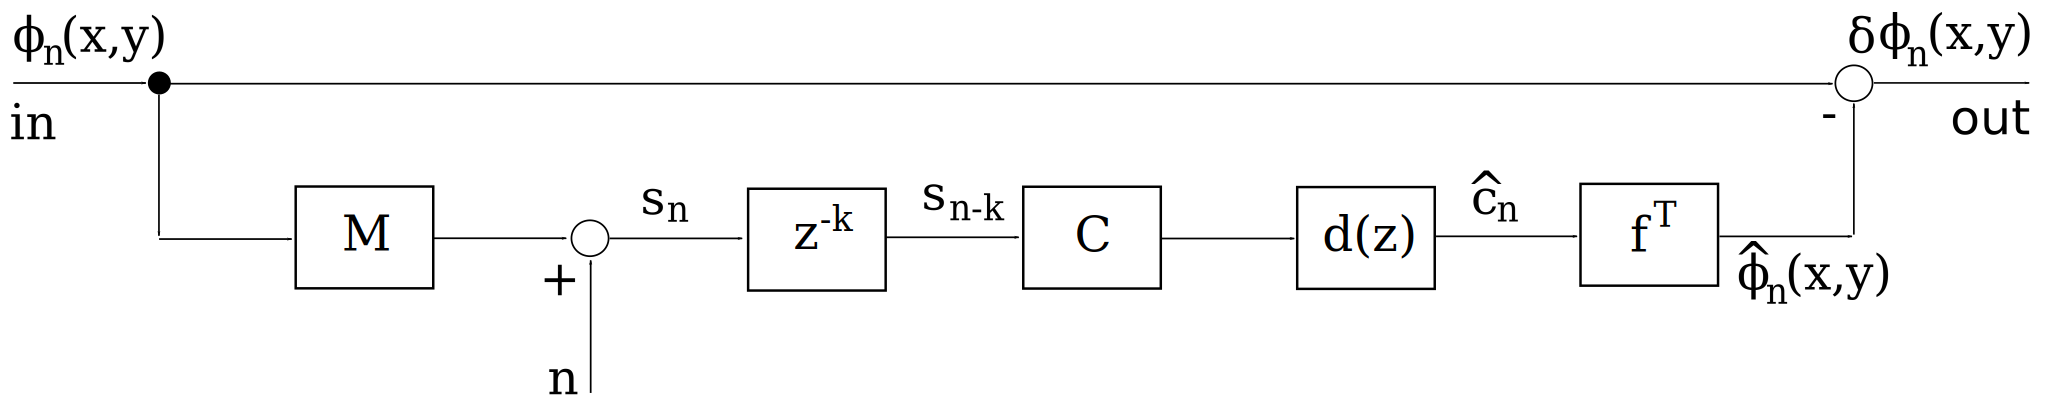
\includegraphics[width = 0.9\textwidth]{Forward.png} \\
 (a) \\
 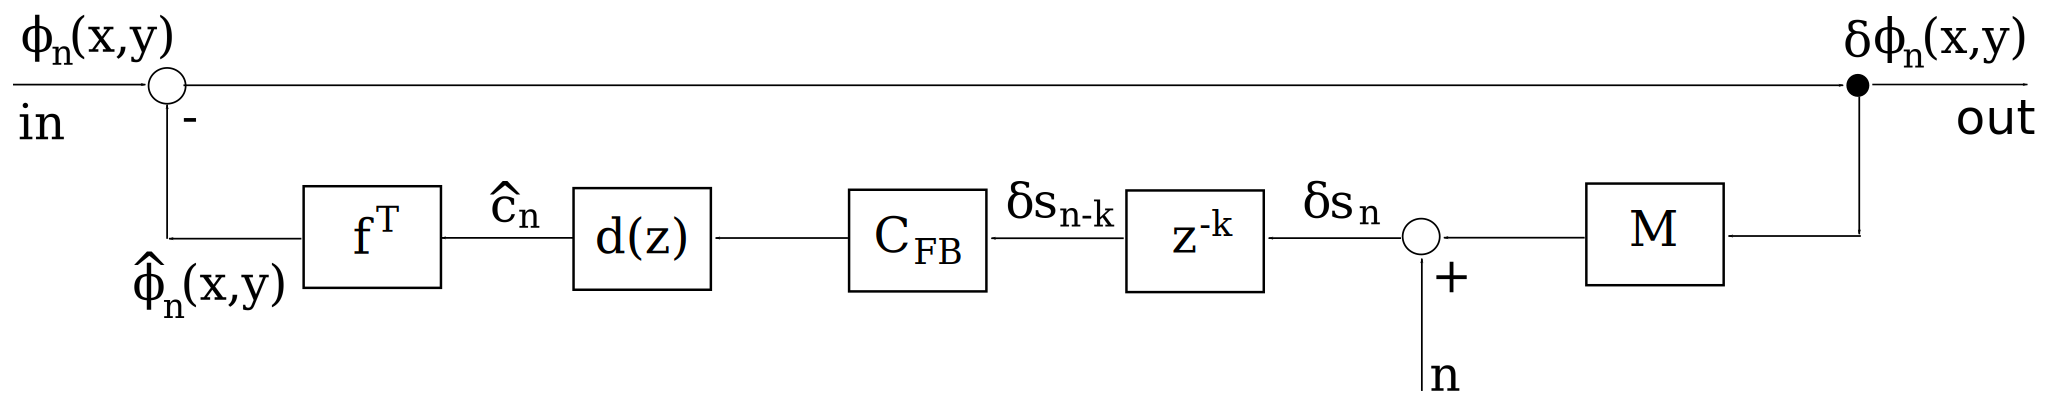
\includegraphics[width = 0.9\textwidth]{Back.png} \\
 (b) \\
\end{tabular}
\end{center}
\caption{Open-loop (a) and closed-loop (b) AO controller block diagrams.}
\label{fig:forward-back}
\end{figure}

Simplified signal block diagrams for an AO system in open-loop and closed-loop
configurations are shown on Fig. \ref{fig:forward-back}.
The system dynamics are modeled by adding: 1)
$k$-step signal delay element with $z$-domain transfer function $z^{-k}$ to
account for delays in sensor and controller; 2) a filter with $z$-domain
transfer function (matrix) $d(z)$ to account for the DM dynamic
effects. It is possible to derive a relationship between the open-loop (or
\emph{feedforward})
reconstructor $\mathcal{C}$ and the closed-loop (or \emph{feedback}) one
$\mathcal{C}_{FB}$ by noticing that, to deliver the same output signal, it
should be
\begin{equation} \label{eq:open-to-close}
  \mathcal{C} \bm{s} = \mathcal{C}_{FB} \delta \bm{s}.
\end{equation}
From the diagrams:
\begin{equation} \label{eq:sopen-to-sclose}
	\delta \bm{s}(z) = \bm{s}(z) - z^{-k} d(z) \mathcal{M} ( \bm{f}^{T}
	\mathcal{C}_{FB} \delta \bm{s}(z) )
\end{equation}
$$
  = \bm{s}(z) - z^{-k} d(z) \mathcal{DC}_{FB} \delta \bm{s}(z),
$$
where $\mathcal{D} = \mathcal{M} (\bm{f}^{T})$ is the \emph{poke matrix}
\index{poke matrix}
relating action of each DM influence function on the WFS measurements.
Substitution of Eq. (\ref{eq:sopen-to-sclose}) into Eq.
(\ref{eq:open-to-close}) yields
\begin{equation} \label{eq:fw-to-fb}
	\mathcal{C}_{FB} = \mathcal{C}
	( \mathcal{I} - z^{-1} d(z) \mathcal{CD} )^{-1}.
\end{equation}

The transfers from input wavefront phase $\phi(n)$ to the AO system
residual phase error $\delta \phi(n)$ (\emph{error rejection transfer
function}): \index{error rejection transfer function} for the feedforward and
feedback controllers shown on Fig. \ref{fig:forward-back} are:
\begin{equation} \label{eq:forward-transfer}
	(\phi \rightarrow \delta \phi)(z) =
	\mathcal{I} -
	z^{-k} d(z) \mathcal{D} \mathcal{C};
\end{equation}
\begin{equation} \label{eq:feedback-transfer}
	(\phi \rightarrow \delta \phi)_{FB}(z) =
	( \mathcal{I}+z^{-k} d(z) \mathcal{D} \mathcal{C}_{FB} )^{-1}.
\end{equation}

The open-loop reconstructor $\mathcal{C}$ can also
be used directly in the \emph{pseudo open-loop} \index{pseudo
open-loop} (POL) setting of the closed-loop control when the open-loop
measurement is approximately restored
through an internal model for the DM. In the case of linear internal model the
approximate (pseudo) open-loop WFS measurement $\hat{\bm{s}}$ is
\begin{equation} \label{eq:wfs-restoration}
	\hat{\bm{s}} = \delta \bm{s} + \mathcal{D} \bm{c}.
\end{equation}
Block diagram for a dynamic MMSE controller working in the POL regime is
shown on Fig. \ref{fig:POL}. The integrator/corrector filter $g(z)$ is used to
produce the absolute DM
commands from differential ones in a way ensuring system stability and dynamic
error minimization.
\begin{figure}[htp]
\begin{center}
 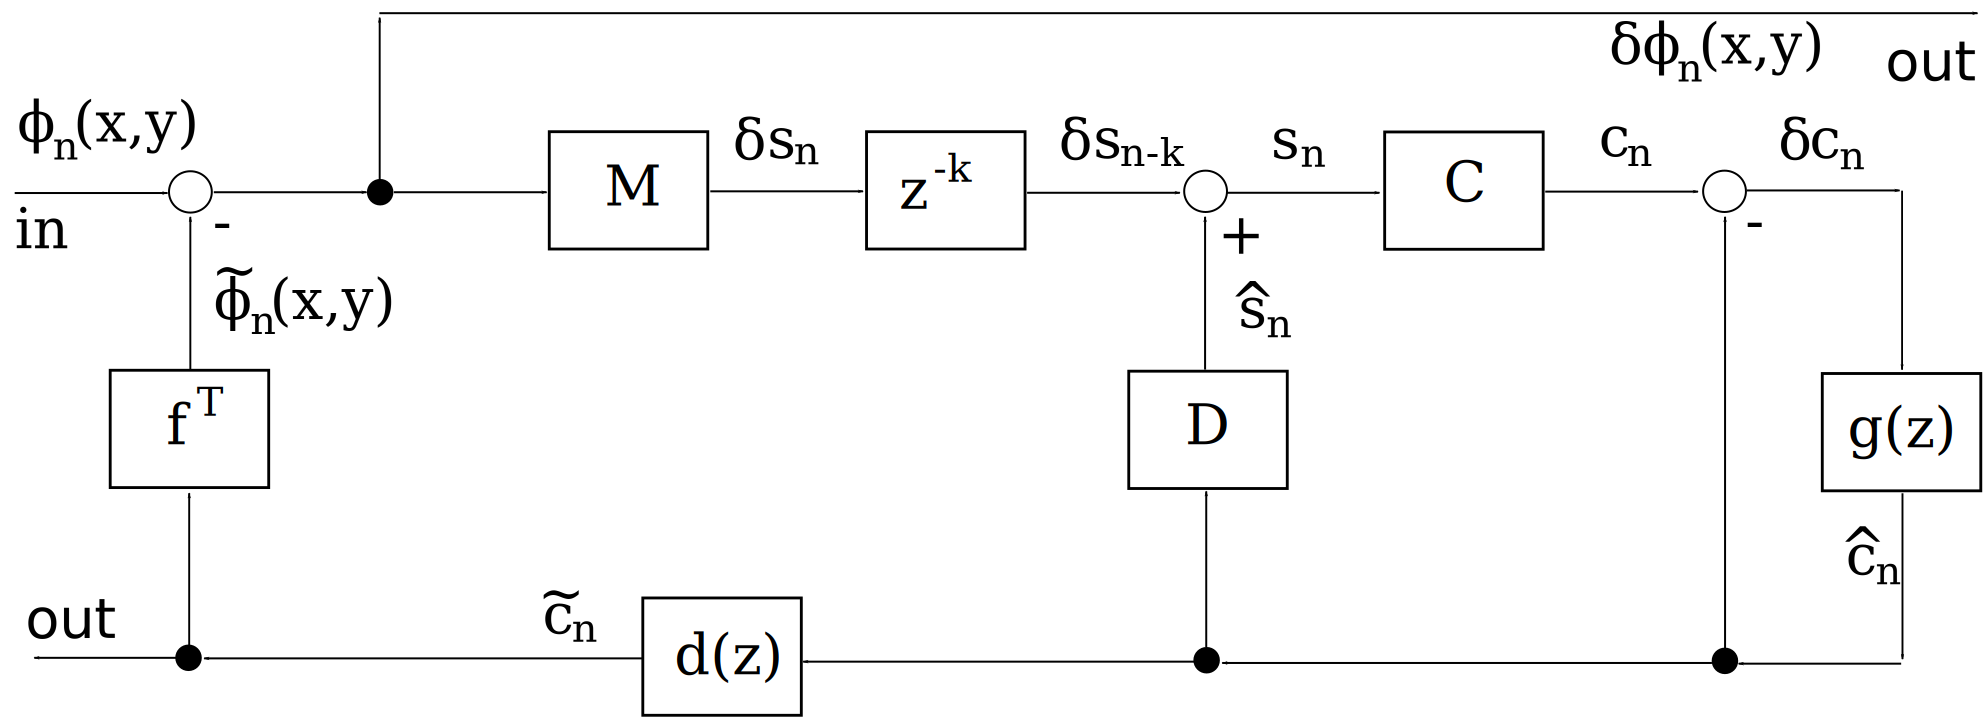
\includegraphics[width = 0.8\textwidth]{POL.png}
\end{center}
\caption{Pseudo Open-Loop MMSE controller block diagram.}
\label{fig:POL}
\end{figure}

The set of dynamic equations for the POL controller is:
\begin{align}
  \texttt{(pseudo open-loop measurement)} \nonumber \\
	\bm{s}(n) = \delta \bm{s}(n-k) + \hat{\bm{s}}(n); \label{eq:POL-meas} \\
	\texttt{(pseudo open-loop command)} \nonumber \\
  \bm{c}(n) = \mathcal{C} \bm{s}(n); \label{eq:POL-est} \\
  \texttt{(command increment)} \nonumber \\
  \delta \bm{c} = \bm{c}(n) - \hat{\bm{c}}(n); \\
  \texttt{(integrator/corrector state space equations, see Appendix
  \ref{app:DF})} \nonumber \\
  \bm{x}^{g}(i+1) = \mathcal{A}^{g} \bm{x}^{g}(n) +
                    \mathcal{B}^{g} \delta \bm{c}(n), \\
  \hat{\bm{c}}(n) = \mathcal{C}^{g} \bm{x}^{g}(n) +
                    \mathcal{D}^{g} \delta \bm{c}(n); \\
  \texttt{(pseudo open-loop measurement estimate)} \nonumber \\
  \hat{\bm{s}}(n) = \mathcal{D} \hat{\bm{c}}(n).
\end{align}
Two important transfer functions (matrices) can be derived from the Fig.
\ref{fig:POL} diagram: 1) the transfer from WFS output $\delta \bm{s}(n)$ to
controller output $\hat{\bm{c}}(n)$ (\emph{controller transfer function}):
\index{controller transfer function}
\begin{equation} \label{eq:WFS-to-Control}
	(\delta \bm{s} \rightarrow \hat{\bm{c}})_{POL}(z) =
	z^{-2} g(z) \left[ \mathcal{I} +
	g(z) (\mathcal{I}-\mathcal{RD}) \right]^{-1} \mathcal{C},
\end{equation}
and 2) the error rejection transfer function:
\begin{equation} \label{eq:phase-to-error}
	(\phi \rightarrow \delta \phi)_{POL}(z) =
	\left[ \mathcal{I} + d(z) \bm{f}^{T}
	(\delta \bm{s} \rightarrow \hat{\bm{c}})_{POL}(z) \mathcal{D} \right]^{-1}.
\end{equation}

Being formally equivalent, feedforward, feedback and POL controllers have
different stability and error propagation properties.

\subsection{Tomographic MMSE reconstructor}
\label{subsec:MMSE-tomo}

\mbox{}

A generalization of the single-conjugate AO control is the \emph{star-oriented
tomography}. \index{star-oriented tomography} The AO control problem is
restated as:
\begin{itemize}
  \item Given is a set of thin phase screens (PS)
  $\{ \phi^{t}_{PS}(\bm{x}) \}_{t=1}^{\#PS}$
  located at a number of altitudes above the telescope and representing the
  atmospheric
  turbulence on the path from a light sources to the telescope aperture.

  \item Likewise, given is a set of phase screens $\{ \phi^{m}_{DM}(\bm{x})
  \}_{m=1}^{\#DM}$ representing the corrections by several DMs that are
  conjugated to a number of altitudes above the telescope. Each DM phase
  screen is a linear combination of the DM influence functions:
	\begin{equation} \label{eq:mcao-dm-inf}
		\phi^{m}_{DM}(\bm{x}) = \bm{f}_{m} (\bm{x}) \bm{c}_{m},
	\end{equation}
	where $\bm{f}_{m} (\bm{x})$ are the $m^{th}$ DM influence function set,
	$\bm{c}_{m}$ is the $m^{th}$ DM control command vector.

  \item There are $\#TAR$ scientific targets to be imaged. Associated with
  each target and each PS or DM is a set
  $( \{ \mathcal{T}^{PS}_{lt} \}_{l=1,t=1}^{\#TAR,\#PS},
     \{ \mathcal{T}^{DM}_{lm} \}_{l=1,m=1}^{\#TAR,\#DM} )$
  of the \emph{propagation operators}
  \index{propagation operator} that map PS or DM phase distributions to the
  wavefront phase distribution in the telescope entrance pupil. With
  assumption that these operators are linear, which is justified for weak
  turbulence, the phase from $l^{th}$ light source in the entrance pupil due to
  all PS phase distortions and all DM phase corrections is
  \begin{equation} \label{eq:mcao-pupil-phase}
    \delta \phi^{l}_{0}(\bm{x}) =
    \sum_{t=1}^{\#PS}
    \mathcal{T}^{PS}_{lt}(\phi_{PS}^{t}(\bm{x})) -
    \sum_{m=1}^{\#DM}
    \mathcal{T}^{DM}_{lm}(\phi_{DM}^{m}(\bm{x})),
    \,\, l = 1,...,\#TAR.
	\end{equation}

	\item Likewise, there are $\#REF$ reference sources feeding light to
	wavefront sensors conjugated to the telescope entrance pupil. Associated
	with the reference sources as well as the PSs and DMs are the propagation
	operators
	$( \{ \mathcal{R}^{PS}_{st} \}_{s=1,t=1}^{\#REF,\#PS},
     \{ \mathcal{R}^{DM}_{sm} \}_{s=1,m=1}^{\#REF,\#DM} )$
	mapping PS or DM phase distributions to the
  wavefront phase distribution in the sensor conjugate exit pupils. The
  closed-loop phase distribution on an $s^{th}$ sensor due to all PS phase
  distortions and all DM phase corrections is
  \begin{equation} \label{eq:mcao-sensor-phase}
    \delta \phi^{s}(\bm{x}) =
    \sum_{t=1}^{\#PS}
    \mathcal{R}^{PS}_{st}(\phi_{PS}^{t}(\bm{x})) -
    \sum_{m=1}^{\#DM}
    \mathcal{R}^{DM}_{sm}(\phi_{DM}^{t}(\bm{x})),
    \,\, s = 1,...,\#REF.
	\end{equation}
	Correspondingly, the $s^{th}$ sensor (closed-loop) readouts are
	\begin{equation} \label{eq:mcao-sensor-read}
		\delta \bm{s}_{s} = \mathcal{M}_{s} (\delta \phi^{s}(\bm{x})),
	\end{equation}
	where $\mathcal{M}_{s}$ is the measurement opertor associated with $s^{th}$
	sensor.

	\item The goal of the tomographic AO control is: given a set of sensor
	measurements $\bm{s} = \{ \bm{s}_{s} \}_{s=1}^{\#REF}$ find the commands
	on all the DMs such that to minimize
	\begin{equation} \label{eq:mcao-cost}
		\langle J \rangle_{\phi,n} =
	  \sum_{l=1}^{\#TAR}
	  w_{l} \langle || \delta \phi_{0}^{l} ||^{2} \,|\, \bm{s} \rangle_{\phi,n},
	  \,\, \sum_{l=1}^{\#TAR} w_{l} = 1,
	\end{equation}
	where $\bm{w} = \{ w_{l} \}_{l=1}^{\#TAR}$ is the set of \emph{target
	direction relative
	weights} \index{target direction weights} and the conditional expectation
	(estimator) is taken over the joint
	statistics of the turbulence layers and the sensor noise.

\end{itemize}

For compactness of notation we introduce the following concatenations:
\begin{itemize}
	\item Propagation operator matrices
	\begin{equation} \label{eq:ps-tar-matrix}
		\mathcal{T}^{PS} = \{ \mathcal{T}^{PS}_{lt} \}_{l=1,t=1}^{\#TAR,\#PS};
	\end{equation}
	\begin{equation} \label{eq:dm-tar-matrix}
		\mathcal{T}^{DM} = \{ \mathcal{T}^{DM}_{lm} \}_{l=1,m=1}^{\#TAR,\#DM};
	\end{equation}
	\begin{equation} \label{eq:ps-ref-matrix}
		\mathcal{R}^{PS} = \{ \mathcal{R}^{PS}_{st} \}_{s=1,t=1}^{\#REF,\#PS};
	\end{equation}
	\begin{equation} \label{eq:dm-ref-matrix}
		\mathcal{R}^{DM} = \{ \mathcal{R}^{DM}_{sm} \}_{s=1,m=1}^{\#REF,\#DM}.
	\end{equation}

	\item Phase vectors
	\begin{equation} \label{eq:ps-vector}
    \bm{\phi}_{PS} (\bm{x}) = \{ \phi_{PS}^{t} (\bm{x}) \}_{t=1}^{\#PS};
	\end{equation}
	\begin{equation} \label{eq:dm-vector}
    \bm{\phi}_{DM} (\bm{x}) = \{ \phi_{DM}^{m} (\bm{x}) \}_{m=1}^{\#DM};
	\end{equation}
	\begin{equation} \label{eq:ps-dm-tar-vector}
    \delta \bm{\phi}_{0} (\bm{x}) =
    \{ \delta \phi_{0}^{l} (\bm{x}) \}_{l=1}^{\#TAR};
	\end{equation}
	\begin{equation} \label{eq:ps-dm-ref-vector}
    \delta \bm{\phi} (\bm{x}) =
    \{ \delta \phi^{s} (\bm{x}) \}_{s=1}^{\#REF}.
	\end{equation}

	\item Sensor measurement vector
	\begin{equation} \label{eq:mcao-meas}
		\delta \bm{s} =
		\{  \mathcal{M}_{s} (\delta \phi^{s}(\bm{x})) \}_{s=1}^{\#REF}.
	\end{equation}

	\item DM influence matrix and control command vector
	\begin{equation} \label{eq:mcao-inf}
		\mathcal{F} (\bm{x}) = \texttt{diag} \{ \bm{f}_{m} (\bm{x}) \}_{m=1}^{\#DM};
	\end{equation}
	\begin{equation} \label{eq:mcao-command}
		\bm{c} = \{ \bm{c}_{m} \}_{m=1}^{\#DM}.
	\end{equation}

	\item Target direction weighting matrix
  \begin{equation} \label{eq:direction-weight}
		\mathcal{W} = \texttt{diag} \{ w_{l} \}_{l=1}^{\#TAR},
	\end{equation}
	and the \emph{weighted norm} \index{weighted norm}
	\begin{equation} \label{eq:weighted-norm}
		|| \bm{\phi} ||^{2}_{\mathcal{W}} =
		\sum_{i} w_{i} || \bm{\phi}_{i} ||^{2} =
		[ \bm{\phi}^{T}, \mathcal{W} \bm{\phi} ].
	\end{equation}

\end{itemize}
In this notation the minimization problem for the cost function given in Eq.
(\ref{eq:mcao-cost}) can be written as
\begin{equation} \label{eq:mcao-minimization}
	\hat{\bm{c}} = \arg \min_{\forall \bm{c}}
	\langle
	||
	\mathcal{T}^{PS} (\bm{\phi}_{PS}) -
	\mathcal{T}^{DM} (\mathcal{F}^{T}) \bm{c}
	||^{2}_{\mathcal{W}} \,|\, \bm{s}
	\rangle_{\phi,n},
\end{equation}
which is a tomographic analog of Eq. (\ref{eq:joint-minimization}).

The tomographic analog to the deterministic DM fitting problem is then stated
as: find the control commands $\hat{\bm{c}}$ for all DMs such that
\begin{equation} \label{eq:tomo-dm-fitting}
	\hat{\bm{c}} = \arg \min_{\forall \bm{c}}
	||
	\mathcal{T}^{PS} (\bm{\phi}_{PS}) -
	\mathcal{T}^{DM} (\mathcal{F}^{T}) \bm{c}
	||^{2}_{\mathcal{W}}.
\end{equation}
To derive solution to this problem we first consider the matrix analog to the
orthogonality principle Eq. (\ref{eq:deterministic-orthogonality-principle}).
Replace each influence function $f_{i}(\bm{x})$ with e.g. a finite vector of
its values on the entrance pupil point grid:
$$ f_{i}(\bm{x}) \rightarrow \bm{f}_{i} = \{ f_{i}(\bm{x}_{j}) \}_{j=1,\#PT},
   \,\, i = 1,...,\#ACT. $$
Then $ \bm{f}^{T}(\bm{x}) \bm{c} \rightarrow \mathcal{F}^{T} \bm{c} $, where
$\mathcal{F}^{T} = [\bm{f}_{1} \,...\, \bm{f}_{\#ACT}]$ and the matrix form
of Eq. (\ref{eq:deterministic-orthogonality-principle}) reads as
\begin{equation} \label{eq:matrix-orthogonality-principle}
	\mathcal{F} (\bm{x}_{0} - \mathcal{F}^{T} \bm{c}) = 0,
	\,\, \bm{x}_{0} = \{ \phi_{0}(\bm{x}_{j}) \}_{j}^{\#PT}.
\end{equation}
Applying this to Eq. (\ref{eq:tomo-dm-fitting}) one derives by analogy
\begin{equation} \label{eq:tomo-dm-fit}
  [ ( \mathcal{T}^{DM} (\mathcal{F}^{T}) )^{T},
	    \mathcal{T}^{PS} (\bm{\phi}_{PS}) -
		  \mathcal{T}^{DM} (\mathcal{F}^{T}) \bm{c} ) ]_{\mathcal{W}} = 0
\end{equation}
and
\begin{equation} \label{eq:tomo-dm-fit}
  \hat{\bm{c}} =
  [ (\mathcal{T}^{DM} (\mathcal{F}^{T}))^{T},
		 \mathcal{T}^{DM} (\mathcal{F}^{T}) ]^{-1}_{\mathcal{W}}
  [ (\mathcal{T}^{DM} (\mathcal{F}^{T}))^{T},
		 \mathcal{T}^{PS} (\bm{\phi}_{PS}) ]_{\mathcal{W}},
\end{equation}
where the \emph{weighted Hilbert metric} is defined as
\index{weighted Hilbert metric}
\begin{equation} \label{eq:weighted-Hilbert-metric}
	[\bm{a}(\bm{x}),\bm{b}(\bm{x})]_{\mathcal{W}} =
	[ \bm{a}^{T}(\bm{x}), \mathcal{W} \bm{b}(\bm{x}) ],
\end{equation}
$[*,*]$ is the usual Hilbert space metric. Correspondingly, the controllable
part of the phase in the entrance pupil for all the target directions is
\begin{equation} \label{eq:tomo-controllable}
	\hat{\bm{\phi}}_{0} = \mathcal{T}^{DM} (\mathcal{F}^{T}) \hat{\bm{c}}.
\end{equation}

The tomographic phase estimation problem is stated as: find the estimate of
phase $\tilde{\bm{\phi}}_{0}$ in entrance pupil for all the target
directions such that
\begin{equation} \label{eq:tomo-phase-estimation}
	\tilde{\bm{\phi}}_{0} = \arg \min_{\forall \mathcal{E}}
	\langle
	||
	\mathcal{T}^{PS} (\bm{\phi}_{PS}) -\mathcal{E} \bm{s}
	||^{2}_{\mathcal{W}}
	\rangle_{\phi,n}
\end{equation}
with the solution written by analogy with Eq. (\ref{eq:phase-estimate})
\begin{equation} \label{eq:tomo-phase-estimate}
  \tilde{\bm{\phi}}_{0} =
  \langle
  \mathcal{T}^{PS} (\bm{\phi}_{PS}) \bm{s}^{T}
  \rangle_{\phi,n}
  \langle
  \bm{s} \bm{s}^{T}
  \rangle_{\phi,n}^{-1} \bm{s}.
\end{equation}
Finally, according to the separation principle, the tomographic
reconstructor generates the estimate $\hat{\tilde{\bm{\phi}}}_{0}$ optimal in
the sense of Eq. (\ref{eq:mcao-minimization}) by substitution of Eq.
(\ref{eq:tomo-phase-estimate}) into Eq. (\ref{eq:tomo-dm-fit}) and then into
Eq. (\ref{eq:tomo-controllable}). This completes the description of a general
tomographic star-oriented AO system.

The GMT LTAO system can be described as a group of inter-connected tomographic
AO subsystems. The detailed mapping of the AO control theory developed in the
previous sections onto the GMT LTAO is given in the next section.

\subsection{GMT LTAO sub-systems}
\label{subsec:ltao-sub-systems}

\mbox{}

According to the \emph{split control concept} \index{split control concept}
the entire GMT LTAO system can be viewed as a set of weakly interacting
control sub-systems (feedback loops, see Fig. TBD):
\begin{enumerate}
	\item The \emph{ASM high order LGS-based} (ASM HO LGS) \index{ASM high order
	LGS-based control loop}
	control loop intended to reject high spatial order atmospheric/telescope
	aberrations and using the LGS return for WFS measurements. This channel has
	the following features:
	\begin{itemize}
		\item This channel works in closed-loop behind ASM.
		\item Target is $\phi_{Sc}$ is the wavefront from a scientific object.
		\item Reference is $\phi_{LGS}$ is the wavefront from 6 LGSs.
	  \item The control commands generated in this channel are sent to the ASM.
	  \item The wavefront sensors for this channel are the 6 LGS WFSs.
	  \item The sampling rate is the one of the LGS WFSs.
	\end{itemize}

	\item The \emph{ASM low order NGS-based} (ASM LO NGS) or ``truth'' control
	loop is used to provide low order ASM correction, which is impossible to
	determine from the LGSs. Another possible use of the LO NGS WFS is to sense
	the primary segment differential pistons. \index{ASM low order NGS-based
	control loop} This channel has the following features:
	\begin{itemize}
		\item This channel works in closed-loop behind ASM and OI DM.
		\item Target is the wavefront $\phi_{Sc}$ from a scientific object.
		\item Reference is the wavefront $\phi_{NGS}$ from one NGS.
	  \item The control commands generated by this channel are sent to ASM.
	  \item The wavefront sensor for this channel is the LO NGS WFS (``truth
	  sensor'').
		\item The sampling rate is the one of the LO NGS WFS.
	\end{itemize}

	\item The \emph{ASM tip/tilt NGS-based} (ASM TT NGS) \index{ASM tip/tilt
	NGS-based control loop} control loop
	intended to sense and correct the waveront tip/tilt in the scientific object
	direction using a natural guide star. This channel has
	the following features:
	\begin{itemize}
		\item This channel works in closed-loop behind ASM and OI DM.
		\item Target is the wavefront $\phi_{Sc}$ from a scientific object.
		\item Reference is the wavefront $\phi_{NGS}$ from one NGS.
		\item The control commands generated in this channel are sent to the ASM.
		\item The wavefront sensor for this channel is a quad-cell tip/tilt NGS
		(TT NGS) WFS.
	  \item The sampling rate is the one of the TT WFS.
	\end{itemize}

  \item The \emph{OI DM high order LGS-based} (OI DM HO LGS)
  \index{OI DM high order LGS-based control loop} control loop is for
  correcting the NGS wavefront by the OI DM in order to improve performance of
  the NGS TT channel. This channel has the following features:
  \begin{itemize}
	  \item This channel works in closed-loop behind ASM.
	  \item Target is the wavefront $\phi_{NGS}$ from a NGS.
	  \item Reference is the wavefront $\phi_{LGS}$ from 6 LGSs.
	  \item The control commands generated in this channel are sent to OI DM.
	  \item The wavefront sensors for this channel are the 6 LGS WFSs.
    \item The control algorithm is closed-loop with respect to the ASM but
    open-loop with respect to OI DM.
	  \item The sampling rate is the one of the LGS WFSs.
	\end{itemize}

	\item The \emph{OI DM low order NGS-based} (OI DM LO NGS) control loop is
	to provide the low order OI DM correction, which is not possible to
	determine from the LGSs.  \index{OI DM low order NGS-based control loop}
	This channel has the following features:
	\begin{itemize}
		\item This channel works in closed-loop behind ASM and OI DM.
		\item Target is the wavefront $\phi_{NGS}$ from a NGS.
		\item Reference is the wavefront $\phi_{NGS}$ from the same NGS.
		\item The control commands generated by this channel are sent to OI DM.
	  \item The wavefront sensor for this channel is the LO NGS WFS.
		\item The sampling rate is the one of the LO NGS WFS.
	\end{itemize}

\end{enumerate}

One has also to mention some auxiliary control channels used for or together
with LTAO. They are not based on the standard AO control and use other control
approaches.
\begin{enumerate}
	\item \emph{LGS focus stabilization subsystem} \index{LGS focus stabilization
	subsystem} is used for adjusting the LGS WFS
	module focal plane to follow slow LGS position changes in the sky. This
	channel has the following features:
	\begin{itemize}
		\item The feedback signal is the global focus mode extracted from the 6
		LGS WFS measurements.
		\item The control is applied to a servo actuator moving the whole LGS WFS
		module to adjust to the focus. The controller needs to be optimized to the
		(actuator + LGS module) dynamics.
	\end{itemize}
	\item \emph{LGS pupil de-rotation subsystem} \index{LGS pupil de-rotation
	subsystem} is used for compensation of the exit
	pupil rotation on the LGS module induced by changes in the telescope pointing.
	This channel has the following features:
	\begin{itemize}
		\item The feedback signal for this channel is the correlated part of the
		LGS WFS spot motions.
		\item The control is applied to a servo actuator rotating the whole LGS
		WFS module to adjust to the pupil rotation.
	\end{itemize}
	\item \emph{OI WFS acquisition/image stabilization subsystem} \index{OI WFS
	acquisition/image stabilization subsystem} is used find the NGS
	in the telescope field-of-view, to point the light from an NGS to the
	OI WFS detectors and stabilize it. This channel has the following features:
	\begin{itemize}
		\item An acquisition camera is used to provide a signal to the controller.
		\item The control is applied to a two degree-of-freedom actuator attached
		to the acquisition flat mirror located inside OI WFS module.
		\item The acquisition camera and mirror work in closed-loop regime behind
		ASM and OI DM.
	\end{itemize}
	\item \emph{GMT phasing subsystem} \index{GMT phasing subsystem} is an
	\emph{active optics} system that keeps the telescope aligned, phased and
	shape-stabilized.
\end{enumerate}
The auxiliary control sub-systems do not directly participate in the AO
correction but the errors in these systems become the additional error inputs
for the main AO controllers thus upsetting indirectly the AO system
performance.

In the following subsections details of the subsystem control algorithms are
discussed. We concentrate there on the non-dynamic algorithm versions to
highlight the basic operation flow and the data structures involved. The
algorithm modifications to account for the dynamic effects are postponed to
the later sections. Note, however, that the information about the non-dynamic
algorithms is higly reusable in the dynamic versions.

%!!!!!!
%Let the low order wavefront part to be removed from the wavefront $\bm{x}_{Sc}$
%by the $\mathcal{P}_{HO}$-matrix or extracted from $\bm{x}_{Sc}$ by the
%$\mathcal{P}_{LO}$-matrix can be presented as a linear combination
%$$
  %\bm{x}_{LO} = \sum_{i=1}^{L} w_{i} \bm{q}_{i}
%$$
%of the mutually orthonormal modes $\{ \bm{q}_{i} \}_{i=1}^{L}$, then the
%projection matrices are:
%\begin{eqnarray} \label{eq:l0-ho-projectors}
	%\mathcal{P}_{LO} &=& \mathcal{QQ}^{T}, \\
	%\mathcal{P}_{HO} &=& \mathcal{I} - \mathcal{QQ}^{T}, \\
	%\mathcal{Q} &=& [\bm{q}_{1} \, ... \, \bm{q}_{L}], \,\,
	%\mathcal{Q}^{T} \mathcal{Q} = \mathcal{I}.
%\end{eqnarray}
%In case $\{ \bm{q}_{i} \}_{i=1}^{L}$ are not orthonormal but linearly
%independent, they can be easily orthonormalized by means of the
%QR-decomposition.
%!!!!!! \\

\subsubsection{ASM HO LGS controller algorithm}



\subsubsection{ASM LO NGS controller algorithm}
\subsubsection{ASM TT NGS controller algorithm}
\subsubsection{OI DM HO LGS controller algorithm}
\subsubsection{OI DM LO NGS controller algorithm}

%The OI DM HO LGS controller is a modification of the standard AO algorithm
%with the following changes:
%\begin{enumerate}
	%\item The OI DM HO LGS estimator matrix $\mathcal{E}_{HO,OIDM}$ is computed
	%by Eq. (\ref{eq:estimator}), where the wavefront $\bm{x}_{Sc}$ from a science
	%target is replaced with wavefront $\bm{x}_{NGS}$ from the NGS:
	%\begin{equation} \label{eq:OI-DM-H)-LGS-estimator}
	  %^{ngs}\mathcal{E}_{ho}^{lgs} = ^{NGS}\mathcal{P}_{HO}
	%\end{equation}
	%\item The POL measurement equation (\ref{eq:POL-meas}) is replaced with
	%\begin{equation} \label{eq:POL-OIDM}
		%\bm{s}(n) = \delta \bm{s}(n) + \hat{\bm{s}}_{ASM}(n),
	%\end{equation}
	%where $\delta \bm{s}(n)$ is the LGS WFS closed-loop measurement, same as
	%that for HO ADM LGS controller input,
	%$\hat{\bm{s}}_{ASM}(n)$ is an estimate of LGS WFS measurement due to
	%commands sent to ASM by the HO ASM LGS, LO ASM NGS and TT ASM NGS
	%controllers.
	%\item There is no integrator in the HO OI DM control loop because the LGS
	%WFSs are not behind OI DM. Thus
	%\begin{equation} \label{eq:H)-OIDM-commands}
		%\hat{\bm{c}}_{HO,OIDM} (n) = \mathcal{E}_{HO,OIDM} \bm{s}(n)
	%\end{equation}
	%is the HO open-loop OI DM control command.
	%\item Since OI DM is behind the ASM, the differential command $\delta
	%\hat{\bm{c}}_{OIDM}$ to be sent to OI DM should take into account the ASM
	%correction:
	%\begin{equation} \label{eq:OIDM-balance}
		%\delta \hat{\bm{c}}_{OIDM} = \hat{\bm{c}}_{OIDM} -
		%\hat{\bm{c}}^{ASM}_{OIDM},
	%\end{equation}
	%where $\hat{\bm{c}}^{ASM}_{OIDM}$ is the best fit of the ASM correction
	%wavefront by the OIDM:
	%\begin{equation} \label{eq:ASM-to-OIDM-fit}
		%\hat{\bm{c}}^{ASM}_{OIDM} = \arg \min_{\forall \bm{c}}
		%|\mathcal{F} \hat{\bm{c}}_{ASM} - \mathcal{F}|^{2}
	%\end{equation}
%\end{enumerate}

\subsection{GMT LTAO system fusion}
\label{subsec:ltao-system-fusion}

TBD

\subsection{GMT LTAO system dynamic analysis}
\label{subsec:ltao-dynamics}

TBD

\subsection{GMT LTAO system error and robustness analysis}
\label{subsec:ltao-errors}

TBD
% To be compiled with pdflatex
% This file is to be included into master file via \input command
% Note that there is no \begin{document} \end{document} brackets!

\newpage
\section{Appendix: \\ Matrix derivatives}
\label{sec:MDerivative}

Derivative of linear matrix functional $$\bm{p}^T \mathcal{F} \bm{z}$$
with respect to matrix $\mathcal{F}$
is computed as follows:
\begin{enumerate}
 \item Write the functional in element-wise form:
   $$ f = \bm{p}^T \mathcal{F} \bm{z} =
      \sum_i \sum_j p_i \mathcal{F}_{ij} z_j. $$
 \item Differentiate with respect to $\mathcal{F}_{ij}$:
    $$ \frac{\partial f}{\partial \mathcal{F}_{ij}} = p_i z_j. $$
 \item Thus $$ \frac{\partial}{\partial \mathcal{F}}
 (\bm{p}^T \mathcal{F} \bm{z}) = \bm{p} \bm{z}^T. $$
\end{enumerate}

Derivative of quadratic matrix functional
$$\bm{z}^T \mathcal{F}^T \mathcal{A} \mathcal{F} \bm{z},$$
where $\mathcal{A}$ is
symmetric real valued matrix, with respect to matrix $\mathcal{F}$ is computed
as follows:
\begin{enumerate}
 \item Write the functional in element-wise form:
		$$ f = \bm{z}^T \mathcal{F}^T \mathcal{AF} \bm{z} =
		\sum_{i=1}^m \sum_{l=1}^n \sum_{j=1}^m \sum_{k=1}^n
		\mathcal{F}_{il} \mathcal{F}_{jk} \mathcal{A}_{ij} z_l z_k. $$
 \item Most conveniently, by writing down the above equation for a case of
 small matrix size, say, 2x2, find by inspection that
		$$ \frac{\partial}{\partial \mathcal{F}}
		(\bm{z}^T \mathcal{F}^T \mathcal{AF} \bm{z}) = 2 \mathcal{AF} \bm{zz}^T. $$
\end{enumerate}

Analogously, the derivatives with respect to vector are:
$$ \frac{\partial}{\partial \bm{z}} ( \mathcal{F} \bm{z} ) = \mathcal{F}, $$
$$
	\frac{\partial}{\partial \bm{z}} \bm{z}^{T} \mathcal{F} \bm{z} =
	2 \bm{z}^{T} \mathcal{F}.
$$

% To be compiled with pdflatex
% This file is to be included into master file via \input command
% Note that there is no \begin{document} \end{document} brackets!

\newpage
\section{Appendix: \\ Basic discrete-time digital filter theory}
\label{app:DF}

\mbox{}

Here the basic formulas for the digital linear filter theory are given.

\emph{Definition}: a time-invariant, single-input-single-output (SISO), order N
disctete-time linear digital filter is given by a
linear, order-N difference equation with constant coefficients:
\begin{equation} \label{eq:filter-diff}
	y(i) = \sum_{k=0}^{N} b_{k} u(i-k) - \sum_{k=1}^{N} a_{k} y(i-k), \,\,
	i = 0,...
\end{equation}
where $i$ is \emph{disctete time}, \index{discrete time} $u(i)$ is the
\emph{input sequence}, \index{input sequance} $y(i)$ is the \emph{output
sequence}. \index{output sequence}
The filter in Eq. (\ref{eq:filter-diff}) is called \emph{causal} \index{causal
filter} because
$y(i)$ does not depend on time instances $i+1$ and on. Appying $z$-transform
to Eq. (\ref{eq:filter-diff}) one gets:
$$ y(z) (1+\sum_{k=1}^{N} a_{k} z^{-k}) = u(z) \sum_{k=0}^{N} b_{k} z^{-k}. $$
from where the \emph{transfer function} \index{transfer function} is:
\begin{equation} \label{eq:transfer-function}
	H(z) = \frac{y(z)}{u(z)} = b_{0} + \frac{\sum_{k=1}^{N} \beta_{k} b_{k}
	z^{-k}}{1+\sum_{k=1}^{N} a_{k} z^{-k}},
\end{equation}
$$ \beta_{k} = b_{k} - b_{0} a_{k}. $$
The canonical state-space model
\begin{equation} \label{eq:canonical-state-space}
	\bm{x}(i+1) = \mathcal{A} \bm{x}(i) + \mathcal{B} \bm{u}(i),
\end{equation}
$$ \bm{y}(i) = \mathcal{C} \bm{x}(i) + \mathcal{D} \bm{u}(i) $$
describes the filter in terms of its internal state $\bm{x}(i)$ dynamics. The
first equation is the \emph{state dynamics equation}, \index{state dynamics
equation} the second is the \emph{measurement equation}. \index{measurement
equation}
The state space model parameters for the filter are easily derivable from Eq.
(\ref{eq:transfer-function}):
\begin{equation} \label{eq:state-space-filter}
	\bm{u}(i) = [u(i)],
\end{equation}
$$ \bm{y}(i) = [y(i)], $$
$$ \mathcal{A} = \left[
\begin{array}{ccccc}
	-a_{1} & -a_{2} & \cdots & -a_{N-1} & -a_{N} \\
	1      & 0      & \cdots & 0        & 0      \\
	0      & 1      & \cdots & 0        & 0      \\
	\vdots & \vdots & \ddots & \vdots   & \vdots \\
	0      & 0      & \cdots & 1        & 0      \\
\end{array}
\right] $$
$$ \mathcal{B} = [1 \, \cdots \, 0]^{T}, $$
$$ \mathcal{C} = [\beta_{1} \, \cdots \, \beta_{N}], $$
$$ \mathcal{D} = [b_{0}]. $$
% To be compiled with pdf LaTeX
% This file is to be included into master file via \input command
% Note that there is no \begin{document} \end{document} brackets!

\newpage
\section{Bibliography}
\label{sec:biblio}

\begin{thebibliography}{}

\bibitem{ConanCentroid}
O. Lardiere, R. Conan, R. Clare, C. Bradley, N. Hubin,
``Performance comparison of centroiding algorithms for laser guide star
wavefront sensing with extremely large telescopes,'' \emph{Appl. Opt.},
\textbf{49}, G78-G94 (2010).

\bibitem{WibergMaxGavel1}
D. M. Wiberg, C. E. Max, and D. T. Gavel, ``A spatial
non-dynamic LQG controller: Part 1, Application to
adaptive optics,'' in \emph{Proceedings of the 2004 IEEE
Conference on Decision and Control} (IEEE, 2004), pp.
3326 - 3332.

\bibitem{WibergMaxGavel2}
D. M. Wiberg, C. E. Max, and D. T. Gavel, ``A spatial
non-dynamic LQG controller: Part 2, Theory,'' in
\emph{Proceedings of the 2004 IEEE Conference on Decision and
Control} (IEEE, 2004), pp. 3333 - 3338.

\bibitem{WibergMaxGavel3}
D. M. Wiberg, C. E. Max, and D. T. Gavel, ``Geometric view of adaptive optics
control,'' JOSA A, Vol. 22, pp. 870 - 880 (2004).

\bibitem{Poyneer1}
L. A. Poyneer, B. Macintosh,
``Spatially filtered wave-front sensor for high-order adaptive optics,''
JOSA A, Vol. 21, Issue 5, pp. 810-819 (2004).

\bibitem{GMT-LTAO-CODR}
\emph{Giant Magellan Telescope. Laser Tomography Adaptive Optics. Conceptual
Design Review.} \\
Research School of Astronomy and Astrophysics, The College of
Physical and Mathematical Science, The Australian National University. \\
GMTO Document Number: GMT-01-00140. (2011)

\bibitem{ConanGMTmath}
Rodolphe Conan, \emph{GMT Mathematics Handbook.} Personal communication. \\
rconan@mso.anu.edu.au

\end{thebibliography}


\newpage
\printindex % print word index in the end

\end{document}